\documentclass[11pt,a4paper,polish,thesis]{dcsbook}

\usepackage{indentfirst}
\usepackage{babel}
\usepackage{float}
\setcounter{secnumdepth}{4}
\setcounter{tocdepth}{3}

\usepackage{color}
\newcommand{\JP}[1]{\textcolor{red}{#1}}

\newfloat{Code}{htbp}{myc}

\begin{document}

\university
\institute
\author{Tomasz Boczkowski \and Mateusz Michalak \and Andrzej Płuszka \and Wojciech Rybicki}
\title{GUI4PDDL: Graficzne narzędzie do opisu problemów automatycznego planowania}
\supervisor{dr inż.~Agnieszka Ławrynowicz}
\date{Poznań, 2014}
\maketitle
\frontmatter
\tableofcontents{}

\mainmatter

\hyphenation{naj-po-pu-lar-niej-szym}
\chapter{Wstęp}
\label{sec:wstep}
\section{Wprowadzenie}
Sztuczna inteligencja to dziedzina wywodząca się z informatyki. Jej początki sięgają lat pięćdziesiątych XX wieku. Jeden z pierwszych badaczy,  John McCarthy, określił sztuczną inteligencję jako ,,naukę i technikę tworzącą inteligentne maszyny''. Pomimo zmian, jakie dokonały się w przeciągu kolejnych 60 lat, definicję tę wciąż można uznać za aktualną. Sztuczna inteligencja obejmuje kilka zagadnień, między innymi logikę rozmytą, sieci neuronowe czy planowanie \cite{ai}.

Automatyczne planowanie jest dziedziną sztucznej inteligencji, która zajmuje się realizacją sekwencji akcji oraz strategii \cite{planning}. Innymi słowy, zadaniem automatycznego planowania jest takie pokierwanie akcjami, by ze stanu początkowego dotrzeć do określonego stanu końcowego (celu). Najczęściej wymagany jest również jak najmniejszy czas lub koszt wykonania ułożonego planu. Istnieje kilka powszechnie znanych języków formalnych, umożliwiających wyrażanie problemu automatycznego planowania. Najbardziej znane języki to STRIPS (\textit{Stanford Research Institute Problem Solver}) \cite{strips} oraz PDDL (\textit{Planning Domain Definition Language}) \cite{pddl}, na którym opiera się projekt będący przedmiotem niniejszej pracy.
	
Język PDDL jest jednym z wyspecjalizowanych języków służących do opisu zagadnień związanych z automatycznym planowaniem. Został utworzony z przeznaczeniem na międzynarodowy konkurs planistyczny (IPC - \emph{International Planning Competition \footnote{http://ipc.icaps-conference.org/}}), mający miejsce w 1998 roku. Wzorowany był na innych językach wyspecjalizowanych w automatycznym planowaniu, między innymi na STRIPS'ie. W niektórych częściach języka PDDL można dostrzec podobieństwo do jego wzorca (na przykład w definiowanych akcjach), jednakże posiada on odmienną składnię.   

W celu wydajnego tworzenia oprogramowania, programiści korzystają z rozmaitych narzędzi. Zdarza się jednak, że samo ich wyszukiwanie i instalacja w systemie operacyjnym, zajmuje więcej czasu niż stworzenie programu. Rozwiązaniem są środowiska programistyczne, zapewniające w większości przypadków podstawowe funkcjonalności, oraz możliwość łatwego wyszukiwania i komponowania potrzebnych narzędzi.

\section{Motywacja}
Pomimo stworzenia PDDL, problemem jest znalezienie odpowiedniego, w pełni funkcjonalnego narzędzia. Obecnie dostępne rozwiązania posiadają istotne wady. Są to między innymi brak możliwości pracy z innym systemem  niż Windows, brakiem odpowiedniego formatowania kodu czy nieodpowiednim kolorowaniem składni. Założeniem projektu GUI4PDDL jest rozwiązanie większości niedogodności związanych z pisaniem programów w języku PDDL.

Obecnie istnieją środowiska programistyczne dla wielu języków. Na rysunku \ref{fig:srodowiskoprogramistyczne} przedstawiono środowisko \emph{Code::Blocks}\footnote{http://www.codeblocks.org/}, które jest 
jednym z narzędzi wspomagających programowanie w języku C++.

\begin{figure}[h!]
    \centering
    
    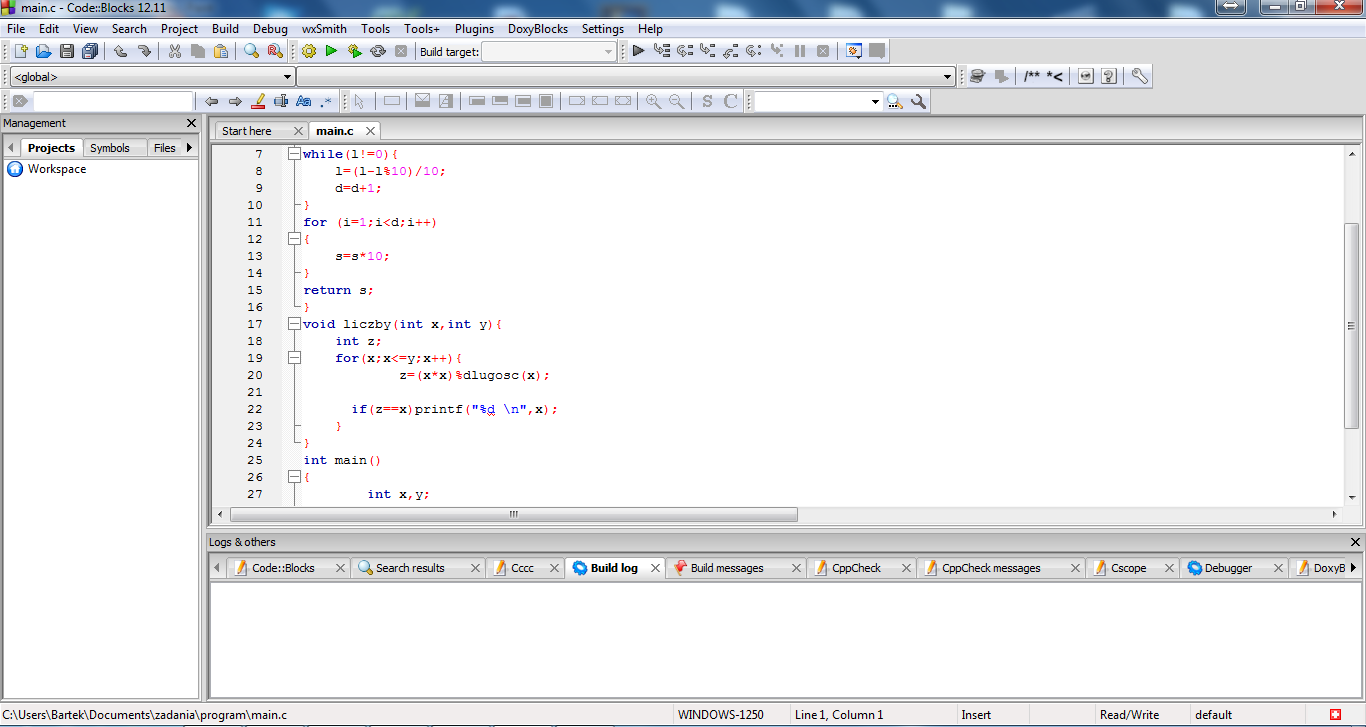
\includegraphics[width=\textwidth]{img/codeblocks}
    \caption{Przykładowe środowisko programistyczne}
    \label{fig:srodowiskoprogramistyczne}
\end{figure}

\section{Cel i zakres pracy}
Celem pracy jest stworzenie graficznego środowiska programistycznego, umożliwiającego pisanie programów w języku PDDL. Środowisko to powinno dostarczać przede wszystkim edytor kodu, zapewniający tworzenie automatycznych wcięć i kolorowanie składni, co pozwala zwiększyć przejrzystość struktury programu. Znaczącymi założeniami edytora są także podpowiadanie składni oraz wykrywanie błędów w kodzie źródłowym, które przyspieszają proces przygotowywania projektu. Dodatkowo, w~związku z wykorzystaniem dużej liczby nawiasów w PDDL, wymagane jest ich dopasowywanie. Dostępna powinna być również możliwość uruchamiania zewnętrznego oprogramowania do wyznaczania planu i przeglądania wyników planowania oraz zarządzania projektami i plikami.  

W pierwszej części drugiego rozdziału (roz \ref{sec:opis}), przedstawiona została problematyka automatycznego planowania. W rozdziale~\ref{sec:jezykpddl} opisany jest język PDDL, a następnie (roz.~\ref{sec:oprogramowanie}) opisano najważniejsze narzędzia służące do przeprowadzania procesu planowania.

Kolejny rozdział (roz. \ref{sec:specyfikacja}) to opis wymagań funkcjonalnych oraz wymagań pozafunkcjonalnych.

Rozdział czwarty podzielony jest na dwie części. W pierwszej z nich (roz. \ref{sec:eclipseśrodowisko})  opisane jest środowisko programistyczne Eclipse, w którym stworzona została wtyczka GUI4PDDL. Jest to również środowisko, na którym docelowo ma działać stworzony projekt. W drugiej części (roz. \ref{sec:antlrśrodowisko}) opisany został generator analizatorów składniowych ANTLR.

W rozdziale \ref{sec:piaty} przedstawiono architekturę tworzonego systemu, uwzględniając jego podział na projekty platformy \emph{Eclipse}. Opisana jest tu również szczegółowa zawartość każdego pakietu głównego projektu.

Następny rozdział (roz. \ref{sec:implementacja}) zawiera szczegółowe przedstawienie implementacji najważniejszych funkcjonalności. Opisane są tu kwestie tworzenia nowego projektu PDDL oraz nowych plików PDDL (roz. \ref{sec:zarzadzanie}).W kolejnej części ukazano zagadnienia związane z~przetwarzaniem kodu PDDL, czyli wykrywanie błędów składniowych i semantycznych oraz podpowiadanie kodu (roz. \ref{sec:przetwarzanie}). Dalej przedstawione są: kolorowanie kodu, automatyczne wcięcia, dopasowanie nawiasów oraz kwestie związane z obsługą podpowiedzi (roz. \ref{sec:edytor}).  Na końcu omówiono współpracę wtyczki z oprogramowaniem wyznaczającym plan, jego konfigurację i uruchamianie, a także przerywanie procesu planowania (roz. \ref{sec:wspolpraca}).

W rozdziale \ref{sec:testy} opisane są testy jednostkowe kodu oraz gramatyk formalnych. Dodatkowo przedstawiono testy akceptacyjne.

W ostatnim rozdziale \ref{sec:podsumowanie} zawarte jest podsumowanie pracy. W dodatku A opisana jest zawartość płyty CD dołączonej do pracy. Na końcu zawarta została bibliografia.
\section{Podział zadań}
W niniejszym podrozdziale zawarty jest zadań, wykonanych przez poszczególne osoby z grupy.\\\\
\begin{description}
  \item[Tomasz Boczkowski] \hfill 
  \begin{itemize}
\item Moduł analizy kodu PDDL
\item Wykrywanie błędów składniowych i semantycznych
\item Podpowiadanie składni
\item Praca pisemna, rozdziały: \ref{sec:antlrśrodowisko}, \ref{sec:przetwarzanie}, \ref{sec:podsumowanie}
\end{itemize}
  \item[Mateusz Michalak] \hfill 
    \begin{itemize}
\item Testy jednostkowe i integracyjne tworzonego oprogramowania
\item Witryna internetowa
\item Praca pisemna, rozdziały: \ref{sec:wstep}, \ref{sec:drugi}, \ref{sec:testy}
\end{itemize}
  \item[Wojciech Rybicki] \hfill 
    \begin{itemize}
\item Integracja wtyczki z istniejącymi narzędziami automatycznego planowania
\item Moduł do przeglądania danych wyjściowych
\item Praca pisemna, rozdziały: \ref{sec:piaty}, \ref{sec:wspolpraca}
\end{itemize}
  \item[Andrzej Płuszka] \hfill 
    \begin{itemize}
\item Edytor kodu PDDL i jego integracja z środowiskeim \textit{Eclipse}
\item Kolorowanie i podpowiadanie składni
\item Praca pisemna, rozdziały: \ref{sec:specyfikacja}, \ref{sec:eclipseśrodowisko}, \ref{sec:zarzadzanie}, \ref{sec:edytor}
\end{itemize}
\end{description}





\hyphenation{wnio-sko-wa-nie}
\chapter{Problematyka automatycznego planowania}
 \section{Opis dziedziny}
Automatyczne planowanie to poddziedzina sztucznej inteligencji, która dotyczy wykonywania sekwencji akcji, realizacji strategii lub generowania planów, prowadzących do określonego wyniku \JP{tu cytowanie}.

Każdy problem automatycznego planowania zawiera stan początkowy oraz stan końcowy. W stanie początkowym określone są wszystkie wartości zmiennych (stany poszczególnych obiektów) jakie aktualnie zawarte są w problemie, a które mają zostać zmienione podczas wykonania planu. W stanie końcowym sformułowane są wartości zmiennych, których osiągniecie jest głównym zadaniem planu. Ponad to problemy automatycznego planowania zawierają zdefiniowane akcje\JP{operatory}, umożliwiające zmianę stanów\JP{chyba: "zmianę stanu" albo "przechodzenie pomiędzy stanami", ponieważ operator albo zmienia stan systemu albo przechodzi z jednego stanu do innego (zależy jak na to patrzeć). W każdym razie operator nie modyfikuje wielu stanów jednocześnie.}.  \JP{Ja na zajęciach tłumaczę w ten sposób: operator to ta abstrakcyjna rzecz, którą definiujemy w problemie, a którą można porównać do funkcji w języku imperatywnym, natomiast instancja operatora (czyli operator z przypisanymi wartościami do wszystkich zmiennych) to działanie, ewentualnie akcja i można je porównać do wywołania funkcji w języku imperatywnym. Fajnie by było, gdyby takie rozróżnienie się gdzieś tutaj pojawiło.} Tylko przez podejmowanie akcji plan może zostać wykonany. Wyjątkiem jest sytuacja, w której stan końcowy jest równy stanu początkowemu.

Plany, otrzymywane w wyniku rozwiązywania problemów, można otrzymać dzięki zastosowaniem różnego rodzaju schematów działania. Spośród klasycznych algorytmów, wymienić można między innymi całkowity przegląd stanów, wnioskowanie w tył czy wnioskowanie w przód. Mimo, iż całkowity przegląd stanów zapewni rozwiązanie najlepsze, jest to rzadko stosowane rozwiązanie. Liczba stanów możliwych do osiągnięcia rośnie wykładniczo, co powoduje, że zaplanowanie nawet niezbyt skomplikowanych problemów, może zająć czas, w którym rozwiązanie znacznie przekracza zdatność do użycia. W takim wypadku stosuje się algorytmy mogące zwrócić plany, których wykonanie zajmie więcej czasu, jednak szybkość ich uzyskania znacznie wzrasta. \JP{tu cytowanie, chyba, że byłoby takie samo jak dwa akapity wcześniej}

Pomimo zwracania satysfakcjonujących wyników przez algorytmy klasyczne, wykorzystywane jest również kilka bardziej złożonych rozwiązań. Jednym z nich jest przekształcenie danego problemu automatycznego planowania w inny, a następnie  rozwiązanie go najlepszą znaną metodą.\JP{W inny problem automatycznego planowania czy w inny problem w ogóle? Jaki?} Kolejnym wyjściem są algorytmy probabilistyczne. Polegają one na polepszaniu wyników podczas kolejnych iteracji. Algorytmy te wykonują akcje z określonym prawdopodobieństwem, przez co, może się okazać, że optymalny plan zostanie uzyskany później niż w przypadku pełnego przeglądu stanów, lub nawet nie zostanie uzyskany nigdy. Na ogół jednak, algorytmy probabilistyczne dostarczają wyniki porównywalne z algorytmami klasycznymi, w nie gorszym czasie.

Bardzo często, w celu zademonstrowania czym jest automatyczne planowanie, stosuje się układ złożony z klocków, umiejscowionych w określonej pozycji. Zadaniem algorytmów planowania jest takie ułożenie akcji, aby stan końcowy położenia klocków zgadzał się ze stanem aktualnym. \JP{Co to jest stan aktualny?}

Przykładowo, istnieją 3 klocki, nazwane odpowiednio $x$, $y$, $z$. Każdy z nich może być podniesiony lub umiejscowionym na jednym z dwóch dostępnych miejsc ($M1$, $M2$) lub na innym klocku, pod warunkami, że ten nie jest akurat podniesiony i nic się na nim nie znajduje. Dla danego problemu zdefiniowane zostały akcje \emph{podnieś}, która podnosi dany klocek, oraz \emph{połóż}, dzięki której można umiejscowić klocek na wolnym miejscu lub innym klocku. Stan początkowy zdefiniowany jest następująco: klocek $z$ położony jest na pierwszym miejscu, klocek $y$ położony jest na klocku $z$, a klocek $x$ na klocku $y$. Stan końcowy wygląda tak, że klocek $x$ znajduje się na miejscu drugim, na nim umiejscowiony jest klocek $y$, a z kolei na nim klocek $z$. Inaczej można przedstawić to w języku predykatów:
\\\\
Stan początkowy:
\\\\
\textit{P=\{wolny(x),na(x,y),na(y,z),na(z,M1)\}}
\\\\
Stan końcowy:
\\\\
\textit{K=\{wolny(z),na(z,y),na(y,x),na(x,M2)\}}

Na rysunku \ref{fig:automatyczne-planowanie} przedstawiono graficzne odwzorowanie stanu początkowego i końcowego.\JP{Ten wielki znak zapytania jest całkiem oryginalny ;)}
\begin{figure}[h!]
    \centering
    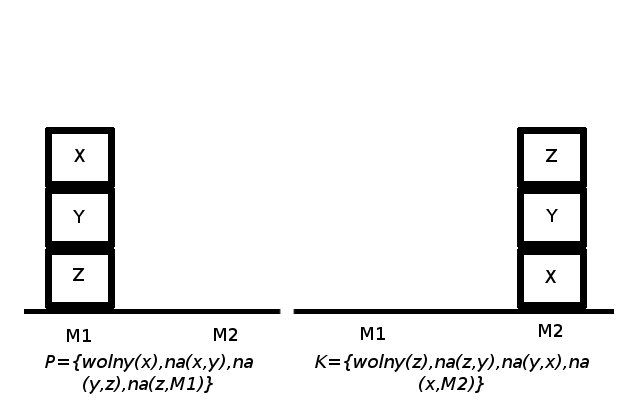
\includegraphics[width=0.5\textwidth]{img/rys2,1}
    \caption{Graficzna reprezentacja stanu początkowego i końcowego}
    \label{fig:automatyczne-planowanie}
\end{figure}


\section{Język PDDL}
W celu polepszenia wydajności automatycznego planowania, stworzone zostało kilka formalnych języków. Najpopularniejsze z nich to STRIPS (ang. \textit{\textbf{St}anford \textbf{R}esearch \textbf{I}nstitute \textbf{P}roblem \textbf{S}olver}) \JP{tu cytowanie}, ADL (ang. \textit{Action description language}) \JP{tu cytowanie} oraz PDDL (ang. \textit{Planning Domain Definition Language}) \JP{tu cytowanie}. PDDL, który stworzony został najpóźniej, jest wzorowany na dwóch pozostałych językach. Został utworzony przez Drew McDermott'a w roku 1998. Celem jego stworzenia był Międzynarodowy konkurs planistyczny (ang. \textit{International Planning Competition}),który bez odpowiedniego narzędzia nie mógłby się odbyć.

Od pojawienia się pierwszej wersji języka w roku 1998, jest on systematycznie rozwijany. Kolejne wersje 2.1, 2.2, 3.0, oraz najnowsza 3.1 zostały użyte na międzynarodowych konkursach w latach 2002, 2004, 2006, 2008. Oprócz standardowych wersji języka, rozwijane są inne, niezależne warianty. Pośród nich znajdują się między innymi PDDL+, w którym zawarto procesy i zdarzenia \JP{tu cytowanie}, Web-PDDL umożliwiający wyrażenie przestrzeni nazw za pomocą URI (ang. \textit{Uniform Resource Identifier}) \JP{tu cytowanie}, czy NDDL (ang. \textit{New Domain Definition Language}), różniący się używaniem zmiennych oraz interwałów zamiast akcji \JP{tu cytowanie, a tak w ogóle to NDDL to chyba nie jest klasyczne planowanie tylko bardziej jakby temporal planning}.

Problemy automatycznego planowania, przedstawione w języku PDDL, są zapisane w dwóch plikach, dziedziny oraz problemu. Poniżej przedstawiono skrócony opis obydwu plików. Składa się on z przedstawienia elementu, krótkiego opisu oraz przykładu.
\\\\\\
Plik dziedziny zawiera:
  \begin{description}
\item[Dziedzina] Definicja dziedziny: \texttt{(define (domain samoloty))}
\item[Rozszerzenie] Dziedzina zawierająca dany wpis dziedziczy wymagania, typy, stałe, akcje, aksjomaty z innej dziedziny: \texttt{(:extends pojazdy) }
\item[Wymagania] Fragmenty języka PDDL wykorzystywane przez opis dziedziny: \texttt{(:requirements :strips :typing)}
\item[Typy] Typy znajdujące się w problemie: \texttt{(:types okno drzwi)}
\item[Stałe] Zdefiniowane stałe \texttt{(:constants pierwsza druga - opona)}
\item[Zmienne dziedzinowe] Zmienne dla dziedzin, które mają zadeklarowe wymaganie \texttt{:expression-evaluation}: \texttt{(:domain-variables zmienna - int)}
\item[Predykaty] Lista predykatów zawartych w domenie (znak \texttt{?} poprzedzający \texttt{x} oznacza, że \texttt{x} jest zmienną) -  \textit{(:predicates (na-lotnisku ?x))}\JP{Przecież to nic nie tłumaczy.}
\item[Pola wieczne] Lista literałów, które są prawdziwe w każdej chwili \texttt{(:timeless literał (nazwa))}
\item[Ograniczenia bezpieczeństwa] Ograniczenia, które muszą pozostać spełnione w każdym punkcie tworzonego planu \texttt{(:safety (:goal (na-lotnisku samolot))}
\item[Operatory] Lista operatorów, których podejmowanie ma zapewnić osiągnięcie celu. Każdy operator zawiera warunki wykonania, parametry oraz efekt, który powinny przynieść: \texttt{(:action laduj :parameters (?s - samolot ?l - lotnisko ?p - powietrze) :precondition (jest-na ?s ?p) :effect (jest-na ?s ?l)) }\\
\end{description}


Plik problemu zawiera:
\begin{description}
\item[Dziedzina] Wskazanie, do której dziedziny odnosi się definiowany problem: \texttt{(:domain loty)}
\item[Wymagania] Opis zawarty w poprzednim akapicie.
\item[Sytuacja] Nazwa sytuacji początkowej: \texttt{(:situation początek)}
\item[Obiekty] Lista obiektów występujących w problemie: \texttt{(:objects drzewo liść)}
\item[Stan początkowy] Opis stanu początkowego problemu w formie listy spełnionych literałów: \texttt{(:init (jest A) (w B hangar))}
\item[Cel] Oczekiwany stan końcowy problemu w formie formuły logicznej, która musi być spełniona: \texttt{(:goal (and (jest A) (w C hangar) (w B lotnisko))}
\item[Długość rozwiązania] Pole stwierdzające, iż istnieje rozwiązanie o podanej długości: \texttt{(:length (:serial 5))}\JP{Czy to raczej nie jest podpowiedź dla planera, że ma szukać rozwiązań o danej długości?}
\end{description}
\begin{Code}
\begin{lstlisting}[language=LISP,frame=single,label=ana_code, caption=Zawartość przykładowego pliku domeny]
(define (domain loty)
(:extends pojazdy)
(:requirements :strips :typing )
(:predicates
	(lotnisko ?m - miejsce)
	(powietrze ?m - miejsce)
	(samolot	?p - pojazd)
	(jest-na ?p - pojazd ?m - miejsce)
)
(:action laduj
	:parameters (?s - samolot ?m - miejsce)
   	:precondition (is-at ?s ?m) 
	:effect (jest-na ?s ?m) 
)
)
\end{lstlisting}
\end{Code}

\begin{Code}
\begin{lstlisting}[language=LISP,frame=single,label=ana_code, caption=Zawartość przykładowego pliku problemu]
(define (problem lotniska-start)
	(:domain lotniska)
	(:situation ladowanie)
	(:init (at B hangar) (at A lotnisko))
	(:goal (and(at A hangar) (at B lotnisko))))
\end{lstlisting}
\end{Code}

\section{Oprogramowanie}
Aby język PDDL mógł spełniać swoją rolę, wymagane są narzędzia służące do planowania. Jednym z takich przyrządów\JP{proszę nie ufać na ślepo słownikowi wyrazów bliskoznacznych} jest \textit{Fast Downward}\JP{URL,cytowanie}, który pozwala na zaplanowanie problemu zapisanego w~jęzeku PDDL w wersji 2.2. Dodatkowo wspiera wymaganie \textit{:action-costs}, używane\JP{wprowadzone} w wersji 3.1. Aplikacja wymaga od użytkownika posiadania\JP{dostępu do} wiersza poleceń oraz prostego edytora tekstu. Do ułożenia planu \textit{Fast Downward} używa heurystyki opartej na algorytmie \textit{Best-First Search}\JP{tylko?}. Na podobnej zasadzie działania oparte są aplikacje \textit{Fast Forward}\JP{URL, cytownaie} oraz \textit{LPG}\JP{URL, cytownaie}.

Kolejny elektroniczny planista\JP{HMM... to jest poważny problem. U nas w Instytucie mianem planisty określa się zazwyczaj scheduler, więc bałbym się użycia tego terminu jako tłumaczenia angielskiego planner. A jeżeli juz, to musi być konsekwentnie używane w całym dokumencie i koniecznie wyjaśnione na początku.} nosi nazwę \textit{Satplan}\JP{URL, cytowanie}. Algorytm wykorzystywany przez ten program spełnia założenia metody automatycznego planowania o takiej samej nazwie: konwertuje daną instancje problemu planowania na instancje problemu spełnialności \JP{spełnialności czego?}, a następnie rozwiązuje wykorzystując odpowiednie schematy działań \JP{???; tak poza tym cytowanie do czegoś co opisuje tę metodę}. Algorytm zawarty w \textit{Satplanie} ma następujący przebieg: utworzenie grafu planistycznego\JP{?} do pewnej długości \textit{k}, zamiana więzi\JP{?} wynikających z grafu na zbiór klauzul,\JP{tu chyba czegoś brakuje, bo zdanie jest gramatycznie niespójne} używając odpowiedniego algorytmu pozwalającego rozstrzygnąć problem spełnialności, znajduje się odpowiednie rozwiązanie. W przypadku gdy nie można było znaleźć wyniku, zwiększona zostaje wartość \textit{k}. Jeśli jednak rozwiązanie zostało znalezione, transponuje się wynik działania algorytmu do wyniku pierwotnego pierwotnego problemu planowania. Na końcu usuwane są niektóre z niepotrzebnych akcji.

Kolejną aplikacją umożliwiającą rozwiązywanie problemów automatycznego planowania jest Gavs+ (\textit{Game Arena Visualization and Synthesis, Plus!})\JP{URL, cytowanie}, który skupia się na kwestiach związanych z grami. Program ten posiada bibliotekę (\textit{PDDL4J}) umożliwiającą wykonywanie problemów zapisanych w PDDL. Dzięki wbudowanemu interfejsowi Gavs+ umożliwia graficzne prześledzenie wynikowego planu.

Wszystkie opisane tu narzędzia stworzone\JP{opublikowane} zostały na licencji otwartego oprogramowania.

%algorytmy używane przez planery
%satplan
%gavs +

\chapter{Specyfikacja wymagań}
\label{sec:specyfikacja}
\section{Wstęp}
Założeniem projektu było utworzenie lekkiego i wydajnego nardzędzia do programowania w języku PDDL. Dodatkowym ważnym wymaganiem było wsparcie zewnętrznego planera FastDownward oraz możliwe dalsze rozwijanie aplikacji w kiedunku innych planerów. Aplikacja powinna pomagać użytkownikowi w utworzeniu plików PDDL, a później w zarządzaniu kodem. Kluczowym elementem zarządzania kodem jest wykrywanie błędów oraz wyświetlenie kodu w czytelnej formie. Aplikacja ma za zadanie pokolorować kod, oddzielić kluczowe fragmenty i podpowiadać słowa kluczowe, wzorem z popularnych środowisk pracy typu edytory języków Java lub Pascal. Ponadto sama aplikacja miała być łatwo dostępna i łatwa w instalacji, jak również w użytkowaniu.
\section{Wymagania funkcjonalne}
\JP{A nie możnaby kolorowania i wykrywania błędów połączyć w jedno? Coś pokroju: Wspomaganie użytkownika w pracy z edytorem?}
\subsection{Kolorowanie składni}
\begin{tabular}{|p{\textwidth}|}
\hline 
\textbf{Przypadek użycia:} Kolorowanie składni\\
\hline
\textbf{Aktorzy:} Użytkownik\\
\hline
\textbf{Pre:} Użytkownik otwiera pusty dokument\\
\hline
\textbf{Post:} System wyświetla pokolorowany kod\\
\hline
\textbf{Scenariusz główny}\\
\hline
\begin{enumerate}
\item Użytkownik wpisuje ciąg znaków do edytora tekstu.
\item Edytor rozpoznaje typ ciągu znaków.
\item Tekst zostaje pokolorowany na odpowiedni kolor.
\end{enumerate}\\
\hline
\textbf{Rozszerzenia}\\
\hline
\begin{enumerate}
\item[2.a] Ciąg znaków to komentarz.
\item[2.b] Ciąg znaków nie jest komentarzem.
\item[2.b.1] Następuje głębsza analiza znaków.
\end{enumerate}\\
\hline
\end{tabular} 

\subsection{Wykrywanie błędów}
\label{reqErrorDetection}
\begin{tabular}{|p{\textwidth}|}
\hline 
\textbf{Przypadek użycia:} Wykrywanie błędów\\
\hline
\textbf{Aktorzy:} Użytkownik\\
\hline
\textbf{Pre:} Użytkownik wpisuje fragment kodu\\
\hline
\textbf{Post:} System wykrywa i wskazuje błędy w dokumencie\\
\hline
\textbf{Scenariusz główny}\\
\hline
\begin{enumerate}
\item Użytkownik wpisuje kod.
\item Edytor pobiera aktualny stan dokumentu.
\item System sprawdza kod pod kątem gramatycznym i semantycznym.
\end{enumerate}\\
\hline
\\\textbf{Rozszerzenia}\\
\hline
\begin{enumerate}
\item[3.a] System wykrywa błąd. 
\item[3.a.1] W domyślnym oknie błędów pojawia się informacja o błędzie i miejscu.
\item[3.a.2] W oknie edytora błąd zostaje podkreślony.
\item[3.b] System nie wykrywa błędu.
\end{enumerate}\\
\hline
\end{tabular}

\subsection{Podpowiadanie składni}
\label{reqAutocompletion}
\begin{tabular}{|p{\textwidth}|}
\hline 
\textbf{Przypadek użycia:} Podpowiadanie składni\\
\hline
\textbf{Aktorzy:} Użytkownik\\
\hline
\textbf{Pre:} Użytkownik wpisuje ciąg znaków\\
\hline
\textbf{Post:} System pokazuje użytkownikowi możliwe zakończenia podanego ciągu\\
\hline
\textbf{Scenariusz główny}\\
\hline
\begin{enumerate}
\item Użytkownik podaje ciąg znaków lub korzysta z okna podpowiedzi.
\item Edytor pobiera ostatnią sekwencję znaków przed kursorem.
\item Ciąg znaków poddany jest analizie.
\item Edytor wyświetla listę w oknie podpowiedzi.
\item Użytkownik zaznacza wybraną podpowiedź.
\item Edytor wpisuje tekst za kursorem.
\end{enumerate}\\
\hline
\\\textbf{Rozszerzenia}\\
\hline
\begin{enumerate}
\item[3.a] System zwraca listę propozycji zaczynających się na podany ciąg znaków.
\item[3.b] System nie znajduje podpowiedzi i zwraca pustą listę.
\end{enumerate}\\
\hline
\end{tabular}

\subsection{Tworzenie nowego pliku PDDL}
\label{reqAutocompletion}
\begin{tabular}{|p{\textwidth}|}
\hline 
\textbf{Przypadek użycia:} Tworzenie nowego pliku PDDL\\
\hline
\textbf{Aktorzy:} Użytkownik\\
\hline
\textbf{Pre:} Użytkownik chce utworzyć plik PDDL\\
\hline
\textbf{Post:} System otwiera plik z szablonem gotowy do pracy\\
\hline
\textbf{Scenariusz główny}\\
\hline
\begin{enumerate}
\item Użytkownik uruchamia kreatora tworzenia pliku PDDL.
\item System prosi o podanie nazwy pliku.
\item Użytkownik wybiera przeznaczenie pliku.
\item Kreator tworzy nowy plik PDDL z szablonem zgodnym z przeznaczeniem pliku.
\end{enumerate}\\
\hline
\\\textbf{Rozszerzenia}\\
\hline
\begin{enumerate}
\item[3.a] Użytkownik uruchamia kreatora tworzenia niestandardowego pliku.
\item[3.a.1] Użytkownik wybiera typ pliku PDDL z listy propozycji.
\end{enumerate}\\
\hline
\end{tabular}

\subsection{Repozytorium kodu}
\label{reqAutocompletion}
\begin{tabular}{|p{\textwidth}|}
\hline 
\textbf{Przypadek użycia:} Repozytorium kodu\\
\hline
\textbf{Aktorzy:} Użytkownik\\
\hline
\textbf{Pre:} Użytkownik chce zainstalować aplikację\\
\hline
\textbf{Post:} System instaluje aplikację\\
\hline
\textbf{Scenariusz główny}\\
\hline
\begin{enumerate}
\item Użytkownik otwiera okno instalacji dodatkowego oprogramowania Eclipse.
\item Użytkownik wpisuje adres repozytorium.
\item System pokazuje listę dostępnych dodatków z podanego źródła.
\item Użytkownik zaznacza wtyczkę GUI4PDDL do instalacji.
\item System rozpoczyna pobieranie oraz instalację.
\item Użytkownik uruchamia ponownie program Eclipse by ukończyć instalację.
\item Po otwarciu programu ponownie wtyczka widoczna jest na liście aktywnych dodatków Eclipse.
\end{enumerate}\\
\hline
\end{tabular}

\section{Wymagania pozafunkcjonalne}
\subsection*{Funkcjonalność}
Wtyczka \emph{GUI4PDDL} umożliwia użytkownikowi efektywne zarządzanie kodem pisanym w języku \emph{PDDL}. Pomaga w kontrolowaniu zawartości kodu. Wtyczka zbudowana jest jako jeden produkt, zgodnie ze specyfikacją wymaganą przez wtyczki programu \emph{Eclipse}. Zgodnie z polityką twórców Eclipse, \emph{GUI4PDDL} jest zbudowana w pełni modułowo, co umożliwia pełną integrację ze środowiskiem oraz jest łatwa w rozwoju.
\subsection*{Bezpieczeństwo}
Żadne dane nie są wysyłane poza środowisko, dzięki czemu spełnia warunki bezpieczeństwa.
\subsection*{Niezawodność}
Oprogramowanie jest kompletne, dojrzałe. Aplikacja pozbawiona jest błędów, które mogłyby wpłynąć pośrednio lub bezpośrednio na pracę zarówno środowiska programistycznego \emph{Eclipse}, jak i kodu napisanego przez użytkownika. Zdolność do odtworzenia oraz niezawodność zapewnia samo środowisko \emph{Eclipse}, pozwalając na automatyczne odtworzenie kodu z kopii zapasowych w przypadku nieprawidłowego zamknięcia programu.
\subsection*{Użyteczność}
Plugin \emph{GUI4PDDL} wykorzystuje wszelkie formy pomocy dla użytkownika dostępne w środowisku \emph{Eclipse}. Użytkownik jest zawsze w prosty i czytelny sposób poinformowany o stanie swojego kodu oraz o błędach w kodzie. Kolorowanie składni pozwala z łatwością wykryć podstawowe błędy gramatyczne, a automatyczne wcięcia i kolorowe nawiasy umożliwiają szybkie znalezienie braków. Dodatkowo umożliwia intuicyjne korzystanie z wcześniej zdefiniowanych plannerów, wykorzystując np. domyślny przycisk uruchamiania kodu \emph{Eclipse}, co pozwala na szybkie i proste użytkowanie kodu przez użytkownika.
\subsection*{Wydajność}
Aplikacja jest bardzo lekka i pracuje w czasie rzeczywistym. Dzięki multiplatformowości użytkownik może korzystać ze wszystkich funkcji programu w systemach operacyjnych \emph{Windows XP}\ i wyżej oraz we wszystkich dystrybucjach linuksa nowszych od \emph{Ubuntu 10.04} lub porównywalnych.
\subsection*{Łatwość konserwacji}
Kod jest utrzymywany w postaci modułowej. Modułowość wzorowana na innych wtyczkach programu Eclipse pozwala na łatwą i nieograniczoną rozbudowę aplikacji \emph{GUI4PDDL}. Dzięki architekturze modułowej, w przypadku wystąpienia błędów podczas rozszerzania wtyczki, aplikacja nie narusza ważnych elementów środowiska w którym pracuje. Wykorzystując schematy stosowane przez twórców \emph{Eclipse} kod jest stabilny i czytelny, zachowując odpowiednie standardy.



\chapter{Wykorzystane oprogramowanie}
\section{Eclipse}
\JP{Proszę zastąpić deweloperów czymś polskim i wyjaśnić co to są dekoratory}
\subsection{Rys historyczny}
W 2001 roku pojawił się na rynku mało znany projekt typu \emph{otwarte oprogramowanie} – \emph{Eclipse 1.0}. Program ten został opisany jako ,,zintegrowane środowisko deweloperskie do wszystkiego i do niczego w szególności”\JP{źródło cytatu}. W założeniu nie miał to być kolejny zestaw narzędzi, a w pełni skalowanle i rozszerzalne środowisko programistyczne. Razem z programem, udostępniono szereg narzędzi dla deweloperów, umożliwiających rozwijanie projektu. Początkowo Eclipse powstał tylko po to, by dowieść, że można zbudować środowisko rozszerzalne w tak dużym zakresie. Dzięki społeczności, bardzo szybko środowisko to rozwinęło się na wiele języków programowania (ponad 1500 narzędzi w \emph{http://marketplace.eclipse.org} na początku stycznia 2014 roku).

Typowy wizerunek programisty otwartego oprogramowania ukazuje bezinteresownego programistę, nocami pracującego nad poprawą błędów i implementacją własnych pomysłów. W Eclipse, początkowe fragmenty kodu były napisane przez programistów firmy \emph{IBM}. Pracownicy ci dostawali pełne wynagrodzenie za pracę nad otwartym projektem, odpowiadaniem na pytania społeczności, naprawą błędów. Początkowy wkład w rozwój Eclipse miały firmy takie jak \emph{Borland}, \emph{IBM}, \emph{Merant}, \emph{QNX Software Systems}, \emph{Rational Software}, \emph{RedHat}, \emph{SuSE}, a także \emph{TogetherSoft}. Firmy te mogły dzięki temu liczyć na wypuszczenie na rynek programów komercyjnych bazujących na tym środowisku. 

Pierwotnie Eclipse składał się z głównych elementów: \emph{Eclipse Platform}, \emph{Eclipse JDT} oraz \emph{Eclipse PDE}. Eclipse Platform stanowił bazę, środowisko programistyczne. JDT to skrót od \emph{Java Devevelopment Tools} - była to pierwsza większa wtyczka, umożliwiająca zarządzanie kodem Java. Jest ona dostępna do dziś, oczywiście w dużo bardziej zaawansowanej formie niż na początku. Ostatni element, PDE (\emph{Plug-in Development Environment}) to narzędzie do rozwijania środowiska Eclipse. Oferuje ono szereg domyślnych wtyczek, zawiera kreatory tworzenia nowych modułów, a także ogromną i wyczerpującą dokumentację na temat całego środowiska.

Na początku Eclipse było znane jako czysta platforma, dziś jest to zaawansowane środowisko programistyczne z ponad 1500 mniejszymi i większymi rozszerzeniami. W Internecie można znaleźć narzędzia i wtyczki do Eclipse umożliwające pisanie i testowanie kodu niemal w każdym języku programowania.

\subsection{Platforma}

Program Eclipse zbudowany jest w języku \emph{Java}, wymaga więc zainstalowanej Javy na komputerze użytkownika.  Całe środowisko składa się osobnych wtyczek współpracyjących ze sobą, oraz rdzenia samego programu (ang. \emph{Eclipse kernel}). Wtyczka to nic innego, jak plik \emph{JAR} z manifestem, określającym zachowanie i przeznaczenie modułu. W manifestach zawierane są również informacje na temat zależności między wtyczkami:

Przykład zależności między wtyczkami opisanych w pliku plugin.xml
\begin{verbatim}
<requires>
	<import plugin="org.apache.xerces"/>
	<import plugin="org.eclipse.core.resources"/>
	<import plugin="org.eclipse.update.core"/>
	:       :        :
	<import plugin="org.eclipse.text" export="true"/>
	<import plugin="org.eclipse.ui.workbench.texteditor" export="true"/>
	<import plugin="org.eclipse.ui.editors" export="true"/>
</requires>
\end{verbatim}

By zachęcić deweloperów do rozwijania środowiska Eclipse, wymyślono tzw. \emph{Extension Points}. Extension Points to elementy takie jak okna, dekoratory\JP{co?}, menu kontekstowe, kreatory – innymi słowy inne wtyczki, jako że cały Eclipse zbudowany jest modułowo\JP{to wtyczki czy extension points? nic nie rozumiem}. Korzystając z tych punktów można domyślne elementy podmienić własnymi, bardziej rozbudowanymi modułami. Dzięki takiemu rozwiązaniu, rdzenną aplikację można niemal w nieograniczony sposób dostosować do swoich potrzeb.\JP{Trzeba gdzieś odnieść się do rysunku \ref{ana_structure}.}

\JP{czy ten przykład służy czemukolwiek?}
\begin{verbatim}
<extension-point id="decorators" name="%ExtPoint.decorators"
                 schema="schema/decorators.exsd"/>
\end{verbatim}

\begin{figure}[h]
  \centering
    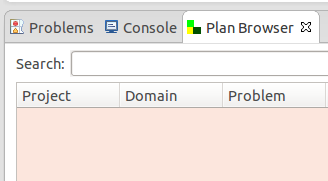
\includegraphics{img/custom-window.png}
    \caption{Dodatkowa zakładka Plan Browser}
    \label{ana_structure}
\end{figure}

Dobrym przykładem jest tutaj całkiem popularne środowisko deweloperskie \emph{Aptana Studio}. Aplikacja ta została zbudowana całkowicie na rdzeniu Eclipse, można więc zauwazyć pewne podobieństwa w układzie okien, modułowości. Mimo podobieństw jest jednak zupełnie inna, ukierunkowana na jedną gałąź programowania – \emph{Web Development}\JP{ten termin angielski na pewno nie jest potrzebny}. Nie wszyscy deweloperzy potrzebują jednak tworzyć całkowicie odrębne oprogramowanie. Eclipse SDK przychodzi z szeregiem domyślnych modułów, takich jak dekoratory, edytory tekstu, paski narzędzi i nawigatory\JP{znam słowo nawigatorzy, ale ono odnosi się do żeglugi. Co to są nawigatory?}. Każdy z tych modułów może zostać zastąpiony własnym lub rozszerzony o pewne funkcjonalności.


\section{ANTLR}
ANTLR (ang. \emph{ANother Tool for Language Recognition}) jest generatorem
analizatorów leksykalnych i składniowych \cite{antlr}.

Narzędzie przetwarza opisy gramatyk języków formalnych w postaci 
zbliżonej do notacji
 Backusa-Naura\JP{tu cytowanie}. Na podstawie specyfikacji generowany jest kod analizatora.
Językami programowania wspieranymi przez ANTLR są między innymi C, C\#, Java
i Python.

Istotną zaletą oprogramowania jest jego prostota użycia. Wygenerowany kod 
jest czytelny i \JP{może zostać łatwo dołączony do tworzonej} łatwo można go dołączyć do własnej aplikacji. Postać plików
wejściowych jest podobna dla wszystkich rodzajów analizatorów. Dodatkowo
istnieją narzędzia wspierające projektowanie i implementację gramatyk
formalnych z wykorzystaniem ANTLR. Należy do nich ANTLRWorks, będące
zintegrowanym środowiskiem programistycznym. Zawiera ono edytor strukturalny,
zintegrowany program do usuwania błędów i moduł do wizualizacji struktur 
danych powstających podczas translacji.

ANTLR został opublikowany wraz z kodem źródłowym na licencji BSD\JP{URL}. Projekt jest
aktywnie rozwijany. Wiele programów zawiera analizatory wygenerowane za pomocą
ANTLR, np. Hibernate\JP{URL}, Jython\JP{URL} i Netbeans\JP{URL}.

\subsection{Przetwarzanie języków formalnych}
Języki formalne, w tym języki programowania, są opisane zbiorem zasad określającym
ich składnię i semantykę. Analiza języka formalnego polega na sprawdzeniu zgodności
danych wejściowych ze specyfikacją języka oraz na wyodrębnieniu części składniowych.
Ponadto podczas analizy mogą zostać wykonane operacje działające na danych zgodnie
z~ich znaczeniem określonym przez reguły semantyczne \cite{compilers}.

\JP{a może zrezygnować z tego wypunktowania i napisać coś pokroju: Wyodrębnia się trzy fazy analizy. Zależności między nimi przedstawione są na rysunku \ref{antlr_phases}}
Wyodrębnia się trzy fazy analizy:
\begin{enumerate}
\item \emph{Analizę leksykalną}.
\item \emph{Analizę składniową}.
\item \emph{Analizę semantyczną}.
\end{enumerate}

\begin{figure}[h]
  \centering
    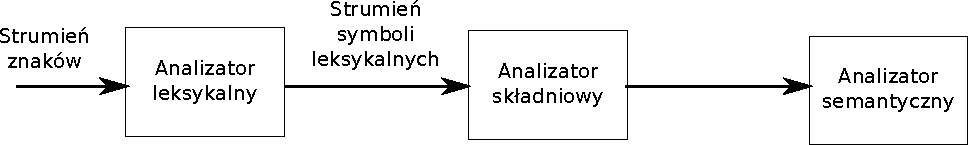
\includegraphics[width=\textwidth]{img/antlr_phases.pdf}
    \caption{Fazy analizy języka formalnego}
    \label{antlr_phases}
\end{figure}

Zależności pomiędzy fazami przedstawia rysunek \ref{antlr_phases}. 

Podczas analizy leksykalnej dane wejściowe są traktowane jako strumień znaków, który
jest odczytywany od strony prawej do lewej. Znaki są grupowane w \emph{symbole leksykalne}, czyli
ciągi posiadające określone znaczenie. Analiza składniowa ma na celu zgrupowanie 
symboli leksykalnych w hierarchiczne struktury,
mające pewne znaczenie.\JP{Z tego fragmentu nie wynika, żeby analiza leksykalna czymś różniła się od składniowej: tak czy siak na końcu są struktury mające znaczenie, co niczego nie mówi} Analiza semantyczna przetwarza dane zgodnie z ich znaczeniem
opisanym przez reguły semantyczne. W~tej fazie zbierane są informacje zawarte w danych.

Reguły języka mogą być opisane językiem naturalnym lub w sposób sformalizowany.
Jednym z formalizmów, odzwierciedlającym hierarchiczną strukturę konstrukcji językowych,
jest \emph{gramatyka bezkontekstowa} \JP{tu cytowanie}. Składa się ona z czterech elementów:

%Pytanie nieuniknięto powtórzenia skłów w definicji
\begin{itemize}
\item Zbioru symboli leksykalnych zwanych \emph{symbolami terminalnymi} lub \emph{terminalami}.
\item Zbioru symboli \emph{nieterminalnych}.
\item Zbioru \emph{produkcji}. Każda produkcja składa się z symbolu nieterminalnego,
  zwanego lewą stroną produkcji, strzałki i ciągu symboli zwanego prawą stroną produkcji.\JP{Czy ta strzałka to jest zaczerpinęta z jakiejś mądrej książki?}
\item Wyznaczonego \emph{symbolu startowego}.
\end{itemize}

Gramatyka \emph{wyprowadza ciąg symboli leksykalnych}, jeżeli wychodząc 
od symbolu startowego i zamieniając symbole nieterminalne na ciągi znajdujące 
się po prawych stronach produkcju, można otrzymać dany ciąg. Sposób, w~jaki
można wyprowadzić dany napis obrazuje \emph{drzewo wyprowadzania}. W~korzeniu drzewa wyprowadzania
znajduje się symbol startowy. Dzieci wierzchołka reprezentującego symbol nieterminalny
zawierają symbole z prawej strony produkcji użytej do jego zastąpienia.

\JP{Proszę przepisać bezosobowo. Ja chyba nie do końca rozumiem czym jest requirementName, bo potem pojawia się :strips jako konkretny przykład. Dobrze by też było, żeby ten przykład był trochę bardziej rozbudowany, bo potem rysunek \ref{antlr_ast} wygląda drętwo.}
\paragraph{Przykład 4.1}
Rozpatrzmy przykład konstrukcji języka PDDL reprezentującej listę wymagań domeny lub problemu.
Składa się ona z otoczonych nawiasami okrągłymi symbolu \texttt{:requirements} oraz
ciągu symboli oznaczających nazwy wymagań. Symbolami terminalnymi są 
\textbf{(}, \textbf{)}, słowo kluczowe \textbf{:requirements} i 
\textbf{requirementName} reprezentujący nazwę wymagania. Poniższa gramatyka opisuje
składnię takiego wyrażenia:

\begin{itemize}
\item requirementsList $\rightarrow$ \textbf{(} \textbf{:requirements} R
\item R $\rightarrow$ \textbf{requirementName} \textbf{)}
\item R $\rightarrow$ \textbf{requirementName} \textbf{R}
\end{itemize}

Dla napisu postaci \texttt{(:requirements :strips)} zostanie
wygenerowany strumień symboli leksykalnych \textbf{( :requirements requirementName )}.
Drzewo wyprowadzania tworzone podczas analizy składniowej jest przedstawione 
na rysunku \ref{antlr_example}

\begin{figure}[h!]
  \centering
    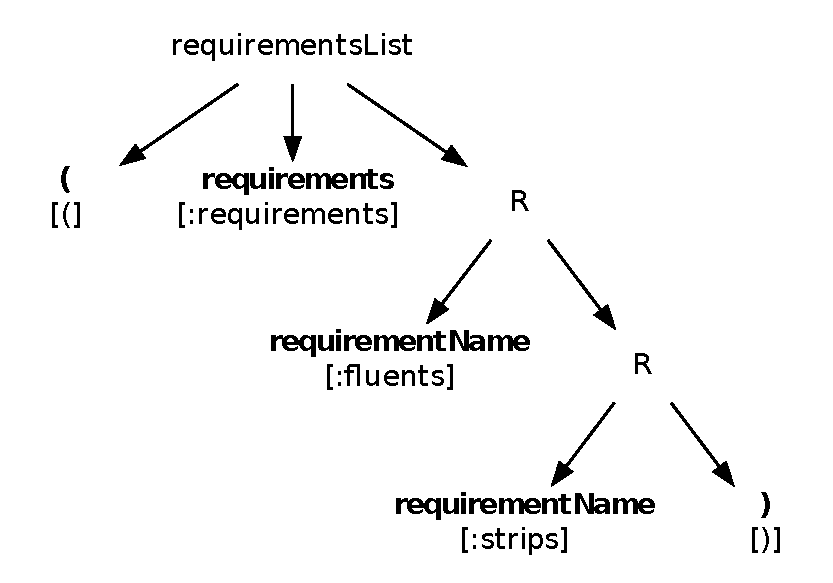
\includegraphics[width=0.7\textwidth]{img/antlr_example.pdf}
    \caption{Drzewo wyprowadzania dla przykładu 12\JP{tu chyba inny numer?}}
    \label{antlr_example}
\end{figure}

\subsection{Metoda LL(*)}
Główną zaletą gramatyk bezkontekstowych jest możliwość automatycznego generowania programów
wykonujących analizę leksykalną i składniową na podstawie gramatyki\JP{tu cytowanie}.

Narzędzie ANTLR generuje analizatory leksykalne i składniowe dla pewnego podzbioru
gramatyk formalnych. Elementy tego podzbioru nazwane są gramatykami LL(*). Metoda 
analizy stosowana w generowanych analizatorach nazwana jest analizą LL(*). 

Analizatory LL(*) należą do klasy analizatorów LL. Wykorzystują one
analizę zstępującą i metodę zejść 
rekurencyjnych. Każdemu nieterminalowi zdefiniowanemu w specyfikacji gramatyki
odpowiada procedura lub metoda\JP{nie bardzo rozumiem to procedura lub metoda. Nie wystarczy jedno z tych słów?}. 

Analiza\JP{jaka? składownia? zstępująca?}, polegająca na konstrukcji drzewa
wyprowadzenia, rozpoczyna się od korzenia. Związany z nim jest symbol 
startowy gramatyki. W każdym kroku analizy wykonywane są następujące czynności:
\JP{Skoro mówimy o drzewie, to chyba jednak właściwszym tłumaczeniem byłyby wierzchołki, a nie węzły}
\begin{enumerate}
\item Wybierany jest pierwszy w porządku, zdefiniowanym przez
  przeszukiwanie wgłąb, węzeł $V$ zawierający symbol nieterminalny $A$.\JP{skąd się wzięło to $A$?}
\item Wybierana jest produkcja mająca po lewej stronie symbol $A$.
\item Jako dzieci węzła $V$ dodawane są węzły związane z symbolami znajdującymi się po prawej
  stronie produkcji z punktu 2.
\end{enumerate}

Typy analizatorów należących do klasy LL różnią się sposobem wyboru produkcji w punkcie 2. 
Analizatory LL(*) są analizatorami przewidującymi. Podejmują one decyzję na
podstawie nieprzetworzonych symboli leksykalnych w strumieniu wejściowym. Liczba
tych symboli nie jest ograniczona. W celu przeglądania strumienia wejściowego 
,,w przód'' tworzone są automaty skończone mogące zawierać cykle.

W odróżnieniu od tradycyjnych gramatyk LL, w~gramatykach LL(*) prawe strony
produkcji dla jednego nieterminala mogą mieć ten sam prefiks. Nie ma więc 
konieczności lewostronnej faktoryzacji, co znacznie ułatwia tworzenie
gramatyk.\JP{Termin lewostronna faktoryzacja musi zniknąć albo być wyjaśniony, bo teraz nie wiadomo o co chodzi.}

\subsection{Abstrakcyjne drzewa składniowe}
% Analizę semantyczną języka opisanego gramatyką bezkontekstową można 
% sprowadzić do obliczania wartości atrybutów przyporządkowanych symbolom
% znajdującym się w drzewie wyprowadzanie. Produkcjom przypisywane są 
% wówczas reguły określające wartości atybutów. Takie podejście 

Formą pośrednią przekazywaną pomiędzy analizatorem składniowym, a semantycznym
może być \emph{abstrakcyjne drzewo składniowe}. Jest to skondensowana postać drzewa
wyprowadzania, składająca się
wyłącznie z węzłów reprezentujących symbole wejściowe. Węzły
wewnętrzne reprezentują słowa kluczowe i operatory, liście -- argumenty.
Abstrakcyjne drzewo składniowe dla przykładu 1\JP{znowu coś z tym numerem jest nie tak} jest przedstawione na rysunku 
\ref{antlr_ast}.

\begin{figure}[h!]
  \centering
    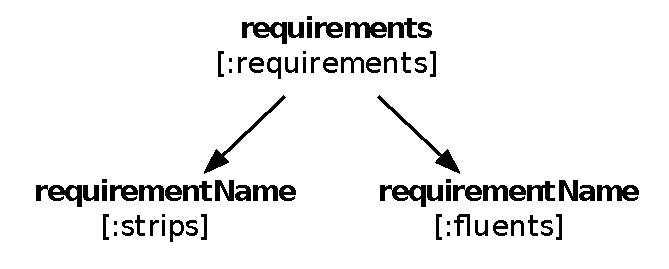
\includegraphics[scale=0.8]{img/antlr_ast.pdf}
    \caption{Abstrakcyjne drzewo składniowe dla przykładu 1\JP{tak jak pisałem wyżej: ten rysunek jest nie dość fascynujący}}
    \label{antlr_ast}
\end{figure}

%Przykład drzewa

Możliwe jest ręczne tworzenie drzewa składniowego za pomocą odpowiednich
reguł semantycznych. Takie podejście proceduralne jest opisane w \cite{compilers}.

Narzędzie ANTLR wspiera tworzenie drzew składniowych. Dodanie
odpowiedniej opcji w specyfikacji analizatora składniowego powoduje automatyczne
wygenerowanie struktury. Poza tym, specyfikacja analizatora składniowego
 może zawierać elementy deklaratywne wpływające na kształt drzewa.


Przetwarzanie abstrakcyjnego drzewa składniowego podczas analizy semantycznej
sprowadza się do jego przechodzenia. Można do tego wykorzystać analizator drzewowy. \JP{Czy drzewowy jest na pewno poprawnym terminem po polsku? Może warto, żeby pojawiła się angielska wersja w nawiasie}
Jest to podprogram generowany przez
ANTLR na podstawie specyfikacji, tak jak analizator składniowy lub leksykalny.
Wprowadzenie analizatorów drzewowych wyróżnia ANTLR na tle innych generatorów
 parserów.  \JP{Czy to się czymś różni od wzorca Visitor? Jeżeli tak, to czym? Jeżeli nie, to warto o tym napisać.}

\subsection{Pliki wejściowe}

Pliki wejściowe ANTLR posiadają rozszerzenie \texttt{.g}. Zawierają one specyfikację
analizatora leksykalnego, składniowego, drzewowego lub połączoną specyfikację
analizatorów leksykalnego i składniowego. 

Specyfikacja analizatorów składa się z listy produkcji, definiujących symbole,
 sekcji opcji konfiguracyjnych oraz kodu dodawanego do generowanego
pliku źródłowego.

W przypadku plików zawierających połączoną specyfikację analizatorów, występuje
podział symboli ze względu na pierwszą literę ich nazwy.
 Symbole, których nazwa rozpoczyna się wielką literą uznawane są
za symbole terminalne. W ich definicjach mogą występować literały i inne
symbole terminalne. Na podstawie reguł definiujących symbole terminalne
tworzony jest analizator leksykalny. Pozostałe reguły tworzą analizator
składniowy.

\JP{Tu bym widział jakiś krótki przykład takiego pliku i/lub odwołanie do odpowiedniego dodatku z omówionym przynajmniej fragmentem takiego kodu ze stworzonego projektu.}

\chapter{Architektura systemu}
\section{Podział na projekty Eclipse}
Ze względu na złożoność oraz zakres wymagań projekt GUI4PDDL podzielono na 6 głównych podprojektów związanych z rozwojem wtyczki (\textit{Plugin Project} lub \textit{Feature Project}) oraz 4 dodatkowe, standardowe projekty Eclipse, służące do testowania istniejących rozwiązań i przechowywania zasobów. Taka struktura pozwala na logiczne oddzielenie najważniejszej części -- implementacji wtyczki od kodu, odpowiedzialnego za możliwość jej integracji oraz związanego z testami. Pozwala to zmniejszyć rozmiar plików pobieranych przy instalacji przez użytkownika, zwłaszcza dodatkowych bibliotek.

Zgodnie z konwencją nazewniczą pakietów języka Java, wszystkie główne projekty mają przedrostek \texttt{pl.poznan.put.cs.gui4pddl}, natomiast w pozostałych obowiązują dowolne nazwy. Dokładna struktura i opis poszczególnych projektów przedstawione są poniżej.

Projekty główne:
\begin{itemize}
\item \textbf{\texttt{pl.poznan.put.cs.gui4pddl}} -- projekt zawierający pełną implementację wtyczki (wersję instalacyjną). Składa się z pakietów odpowiedzialnych za logikę biznesową oraz wszystkie istniejące widoki. Szerszy opis tego projektu znajduje się w rozdziale~\ref{sec:struktura}.
\item \textbf{\texttt{pl.poznan.put.cs.gui4pddl.antlr}} -- projekt zawierający skompilowaną bibliotekę ANTLR, wykorzystywaną w przetwarzaniu gramatyki formalnej języka PDDL.
\item \textbf{\texttt{pl.poznan.put.cs.gui4pddl.feature}} -- projekt \textit{Feature}, umożliwiający połączenie różnych wtyczek w taki sposób, by z zewnątrz były traktowane jako logiczna całość, co ułatwia zarządzanie nimi. Dodatkowo pozwala na uzupełnienie informacji dotyczących wersji, licencji, obsługiwanych systemów operacyjnych itp. Projekt tego typu wymagany jest także w procesie budowania i aktualizacji.

We wtyczce GUI4PDDL grupuje podprojekty \texttt{pl.poznan.put.cs.gui4pddl}\linebreak oraz \texttt{pl.poznan.put.cs.gui4pddl.antlr}, a także udostępnia podstawowe informacje o niej.
\item \textbf{\texttt{pl.poznan.put.cs.gui4pddl.tests}} -- projekt zawierający testy jednostkowe kodu niezwiązanego z interfejsem graficznym (z wykorzystaniem biblioteki \textit{jUnit}) oraz gramatyki formalnej, generowanej przez narzędzie ANTLR, używanej w parserze (z wykorzystaniem biblioteki \textit{gUnit}). Oddzielenie testów od kodu głównego projektu pozwoliło na zmniejszenie wielkości wersji instalacyjnej oraz zredukowanie zależności od dodatkowych bibliotek.
\item \textbf{\texttt{pl.poznan.put.cs.gui4pddl.uitests}} -- projekt zawierający testy jednostkowe interfejsu graficznego, z wykorzystaniem biblioteki \textit{SWTBot}. Biblioteka ta umożliwia przeprowadzenie automatycznych testów akceptacyjnych GUI, stworzonego przy pomocy biblioteki \textit{SWT}.
\item \textbf{\texttt{pl.poznan.put.cs.gui4pddl.update}} -- projekt typu \textit{Update site}, zawierający statyczne pliki, które mogą być umieszczone w określonym miejscu na serwerze. Użytkownicy, korzystając z adresu do tego miejsca mogą pobrać i zainstalować wtyczkę poprzez menedżer aktualizacji. Projekt ten korzysta z wcześniej zdefiniowanego projektu \textit{Feature} oraz zawiera opis wtyczki i kategorię wyświetlone następnie przy instalacji.
\end{itemize}

Pozostałe projekty:
\begin{itemize}
\item \textbf{\texttt{checker}} -- ?
\item \textbf{\texttt{grammar}} -- ?
\item \textbf{\texttt{RubikCube}} -- przykładowy projekt PDDL wykorzystywany podczas rozwijania wtyczki. Zawiera zadanie automatycznego planowania, które z racji swojego charakteru oraz używanego plannera wykonywało się przez znaczny czas, co było pomocne podczas testowania przerywania procesu planowania (roz. \ref{subsec:przerywanie}).
\item \textbf{\texttt{WorldOfBlocks}} -- przykładowy projekt PDDL wykorzystywany podczas rozwijania wtyczki. Zawiera zadanie automatycznego planowania, które z racji swojego charakteru oraz używanego plannera wykonywało się przez krótki czas.
\end{itemize}

\section{Struktura wtyczki}
\label{sec:struktura}

\chapter{Implementacja}
\section{Zarządzanie projektem PDDL}
\subsection{Tworzenie projektu PDDL}
\subsection{Tworzenie nowych plików PDDL}


\section{Przetwarzanie kodu PDDL}
W specyfikacji wymagań zostały zawarte punkty dotyczące wyświetlania błędów znajdujących 
się w pliku PDDL (\ref{reqErrorDetection}) oraz prezentowania listy automatycznych\
podpowiedzi wyrazów (\ref{reqAutocompletion}).
Obie te fukcje oparte są na informacjach zawartych w kodzie źródłowym i związane
z jego analizą.

Modelem informacji umiesczonych w plikach PDDL projektu jest indeks kodu. Jest to
zbiór klas reprezentujących struktury języka PDDL takie jak domeny, problemy, akcje, czy predykaty.
Przy każdej zmianie pliku z kodem źródłowym dokonywana jest jego analiza oraz
aktualizacja indeksu. Ponadto raportowane są błędy występujące w pliku.

Pomiędzy plikami PDDL występują zależności. Aby poprawnie zinterpretować zawartość z plikiem
problemu potrzeba znać zawartość pliku domeny. Powiązanie to jest znacznie prostrze od 
powiązań pomiędzy plikami zawierającymi kod popularnych imperatywnych językach programowania.
Tymniemniej analiza plików PDDL powinna odbywać się w ramach projektu.

W środowisku Eclipse przyjęty jest standardowy sposób rozwiązywania zadania przetwarzania
kodu. Polega on na definicji klasy budowniczego (ang. \emph{builder}). Klasa ta
zawiera kod, który będzie wykonywany przy każdej zmianie zasobu. Zasobem
może być plik lub folder. Budowniczowie
są przypisani do projektu i zawsze działają w jego kontekście.

Budowniczemu przekazywany jest obiekt typu \texttt{IResourceDelta}. Jest to drzewowa
struktura zawierająca zmiany dotyczące zasobów. Na jej podstawie można określić, 
które zasoby zostały dodane, zmodyfikowane lub usunięte. Budowniczy PDDL wywołuje analizator
kodu PDDL dla każdego nowego lub zmienionego pliku. Usunięcie pliku powoduje wykreślenie
odpowiednich informacji z indeksu.

Analizator kodu PDDL został zaimplementowany w klasie PDDLAnalyzer.
Jego struktura została przedstawiona na rysunku \ref{ana_structure}.
Przetwarzany plik PDDL jest poddawany najpierw analizie leksykalnej i zamieniany
na strumień symboli leksykalnych. Następnie, analizator składniowy tworzy abstrakcyjne
drzewo składniowe. Drzewo to poddawane jest analizie semantycznej przez dwa moduły.
Moduł indeksowania kodu tworzy indeks kodu.
Moduł sprawdzania poprawności semantycznej wykrywa błędy na podstawie indeksu oraz
drzewa składniowego. Podprogram obsługi błędów zbiera informacje o błędach występujących
na poszczególnych etapach analizy oraz wyświetla je użytkownikowi.

\begin{figure}[h]
  \centering
    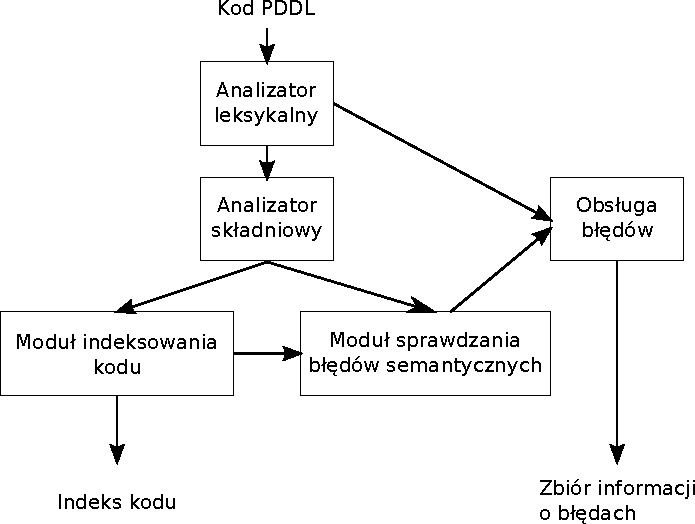
\includegraphics{img/ana_structure.pdf}
    \caption{Struktura analizatora kodu PDDL}
    \label{ana_structure}
\end{figure}

\begin{sloppypar}
Analizator przetwarza pliki w języku PDDL w wersji 1.2 \cite{pddl}. Wspieranymi wymaganiami
są \textbf{:strips}, \textbf{:typing}, \textbf{:disjunctive-preconditions}, \textbf{:equality},
\textbf{:existential-preconditions}, \textbf{:universal-preconditions}, \textbf{:quantified-preconditions},
\textbf{:conditional-effects}, \textbf{:fluents}, \textbf{:adl}.
\end{sloppypar}

\subsection{Analizator leksykaly i składniowy}
Analizator leksykalny i składniowy są automatycznie generowane przez narzędzie ANTLR
na podstawie gramatyki. 

Wykorzystanie generatora analizatorów ma wiele zalet. Nakład pracy poniesiony na
opracowanie gramatyki jest znacznie mniejszy niż przy ręcznej implementacji analizora.
W związku z tym zmniejsza się ryzyko popełnienia błędu. Ponadto, wygenerowane analizatory są 
wydajne. Gramatykę można także przeanalizować pod kątem występowania niejednoznaczności
składniowych
oraz konstrukcji trudnych do analizy. Istotną kwestią jest także to, że
języki zmieniają się w czasie. Dodawane są nowe konstrukcje i zadania. Implementację
bazującą na gramatyce można w łatwy sposób zmienić.

Generator analizatorów ANTLR posiada szereg zalet, które zadecydowały o jego wyborze.
Największe znaczenie miała rozbudowana obsługa błędów w wygenerowanych analizatorach.
Domyślne komunikaty o błędach składniowych są czytelne dla użytkowników końcowych.
Można je też zastąpić własnymi komunikatami. Do ich generacji można wykorzystać tę samą 
informację kontekstową, która służy do utworzenia treści domyślnych komunikatów.
Oprócz tego wykorzystane zostało wbudowane w ANTLR narzędzie do implementacji
terstów jednostkowych gUnit.

Kolejną zaletą narzędzia ANTLR jest dostępność środowiska ANTLRWorks, w którym
rozwijano gramatykę języka PDDL. Udostępnia 
ono edytor kolorujący składnię oraz automatycznie formatujący kod. Możliwe jest
testowe uruchamianie analizatora lub wybranej reguły dla fragmentu kodu PDDL.
Wyświetlana jest wówczas wizualizacja drzewa wyprowadzania. Jest to bardzo przydatne
podczas wyszukiwania błędów gramatyki.

Do implementacji analizatorów wykorzystano specyfikację języka PDDL w wersji 1.2 \cite{pddl}.
Dokument zawiera opis składni za pomocą notacji Backusa-Naura. Na jego podstawie opracowano
gramatykę przetwarzaną przez ANTLR.

\begin{sloppypar}
Pliki związane z analizą programu źródłowego znajdują się w pakiecie 
\texttt{pl.poznan.put.cs.gui4pdddl.parser}.
Plik \texttt{PDDL.g} zawiera połączony opis analizatora
składniowego i leksykalnego.  %Można napisać że duże litery to terminale
Na jego podstawie generowane są klasy \texttt{PDDLLexer} i \texttt{PDDLParser}.
Analizator składniowy tworzy abstrakcyjne drzewo składniowe, używając mechanizmów
wbudowanych w ANTLR.
\end{sloppypar}


Analizatory LL, generowane przez ANTLR, mają własność \emph{prefiksu żywotnego}.
Oznacza to, że błąd jest wykrywany w miejscu, w którym prefiks wejścia nie może
być prefiksem żadnego napisu w danym języku. Miejsce to znajduje się blisko miejsca
wystąpienia błędu.

Kiedy zostanie wykryty błąd, zostaje wywołana procedura obsługi. W klasach 
PDDLLexer i PDDLParser tworzony jest obiekt klasy \emph{PDDLError}. Zawiera
ona informacje o miejscu wystąpienia błędu oraz komunikat diagnostyczny. Użyto
domyślnej treści komunikatów. Obiekt dodawany jest do listy błędów. 

Analiza kodu nie powinna być przerywana przy napotkaniu pierwszego błędu. Takie
działanie byłoby uciążliwe. Dlatego też, po wystąpieniu błędu analizator podejmuje
próbę odzyskania kontroli. Analizator leksykalny przechodzi w tryb paniki. Po napotkaniu 
błędu pomija znaki na wejściu aż do napotkania znaku, który pownien wystąpić.

Domyślna strategia odzyskiwania kontroli przez analizatory składniowe wygenerowane 
za pomocą ANTLR jest opisana w \cite{antlr}. Ze względu na specyfikę języka PDDL
należało wprowadzić pewne poprawki. Pierwsza z nich dotyczy błędów zgłoszonych na końcu pliku.
Zwykle są to błędy wynikające z niedopasowania liczby nawiasów.
Metoda \texttt{recoverFromMismatchedToken} wstawia symbole \textbf{)} tak długo, jak to jest konieczne.
Druga poprawka dotyczy sytuacji, kiedy w miejscu wystąpieniu błędu nie możebyć użyta żadna
z produkcji. Metoda \texttt{recover} próbuje opuścić bieżący poziom zagnieżdżenia.

\begin{Code}
\begin{lstlisting}[language=LISP,frame=single,label=ana_code, caption=Kod PDDL zawierający błąd składniowy]
(define (problem p1)
	(:domain world-of-blocks)
	(:objects a b)
	(:init
		(clear b)
		(on-top c b)
		(on-top b a)
	)
	(:goal
		(ann
			(clear a)
			(on-top a b)
      (on-floor b)
		)
	)
)
\end{lstlisting}
\end{Code}

W kodzie z przykładu \ref{ana_code} znajduje się błąd składniowy. Zamiast słowa kluczowego \textbf{and}
wystąpił w 10 linii ciąg znaków ann. W tym miejscu zostanie zgłoszony błąd. Metoda odzyskiwania kontroli
pominie zagnieżdżone konstrukcje i spowoduje przejście do linii 14.

\subsection{Tworzenie indeksu}
Na podstawie abstrakcyjnego drzewa składniowego tworzony jest indeks kodu. 
Gramatyka opisująca analizator drzewowy znajduje się w pliku \texttt{PDDLModelBuilder.g}.

Klasy będące modelami struktur PDDL i wchodzące w skład indeksu znajdują się w pakiecie
\texttt{pl.poznan.put.cs.gui4pddl.codemodel}. Schemat zależności pomiędzy tymi klasami
przedstawiony jest na rysunku \ref{ana_model}. Wszystkie klasy zawierają metody dostępu
do pól.

\begin{figure}[h]
  \centering
    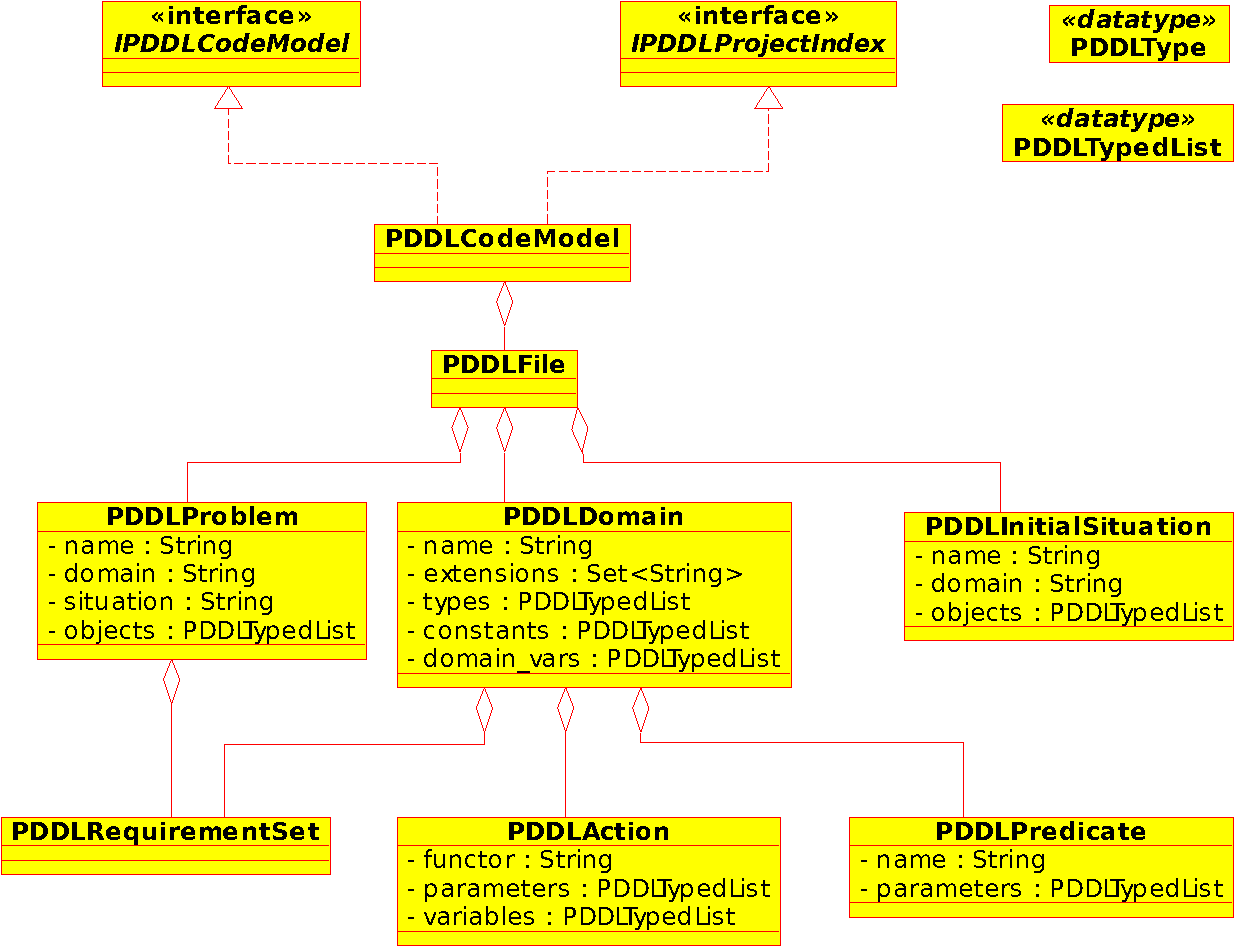
\includegraphics[width=\textwidth]{img/ana_model.pdf}
    \caption{Klasy współtworzące indeks kodu}
    \label{ana_model}
\end{figure}

Indeks kodu przyporządkowany jest projektowi. Znajdują się w nim informacje strukturalne dotyczące każdego
z plików PDDL w projekcie. Istnieją dwa interfejsy związane z indeksem. \texttt{IPDDLCodeModel}
zawiera metody służące do zadawania zapytań i wyszukiwania informacji. W \texttt{IPDDLProjectIndex}
znajdują się metody umożliwiające tworzenie i modyfikacje indeksu.

Klasa \texttt{PDDLCodeModel} implementuje oba interfejsy. Jest ona kolekcją obiektów klasy
\texttt{PDDLFile} reprezentujących pliki PDDL. Każdy z plików może zawierać dowolną liczbę
definicji domen, problemów lub sytuacji początkowych. 

Klasy reprezentujące definicje przechowują część informacji zawartych w pliku. Niektóre
składowe definicji zostały pominięte ze względu na fakt, że są one istotne jedynie 
dla oprogramowania wyznaczającego plan.

Klasa \texttt{PDDLType} reprezentuje typ w języku PDDL. Wspierane są typy proste, typy 
zmienne w czasie \emph{fluent}, oraz typy złożone \emph{either}.
Typ \texttt{PDDLTypedList} odpowiada liście z określeniami typów opisanej w specyfikacji PDDL.
\texttt{PDDLTypedList} stanowi listę wielkości charakterystwanych przez nazwę, będącą 
łańcuchem znaków, oraz typ.

\subsection{Wykrywanie błędów semantycznych}
Do wykrywania błędów semantycznych służy analizator drzewowy, którego gramatyka znajduje się
w pliku \texttt{PDDLSyntaxChecker.g}. Przy przechodzeniu przez abstrakcyjne drzewo składniowe
wykonywane są pewne testy mające na celu sprawdzenie, czy definicje są zgodne z opisem języka.
Wykrywane są następujące błędy semantyczne:
\begin{itemize}
\item nieznana nazwa wymagania.
\item odwołanie do nieistniejącej domeny.
\item odwołanie do nieistniejącego obiektu.
\item odwołanie do nieistniejącego typu.
\item odwołanie do obiektu niezgodne z jego typem.
\item odwołanie do nieistniejącego predykatu.
\item odwołanie do nieistniejącej zmienej.
\item niewykorzystanie zmiennej użytej w definicji akcji.
\end{itemize}

Na pliki w projekcie PDDL nałożone jest dodatkowe ograniczenie. Nazwa pliku zawierającego 
domenę powinna odpowiadać nazwie domeny lub być równa \texttt{domain.pddl}. Dzięki temu 
możliwe jest jednoznaczne znalezienie powiązania pomiędzy domenami a problemami. W przypadku
niespełnienia tego ograniczenia, generowane jest ostrzeżenie.

\subsection{Obsługa błędów}
Krótko o markerach
+Będzie, będzie screenshot.


\subsection{Podpowiadanie kodu}
Automat skończony (para)
Kontekst
I te klasy co zapodają podpowiedz

Podpowiadanie składni wywoływane jest po wpisaniu dowolnej litery, znaku ":" lub po wciśnięciu kombinacji klawiszy Ctrl+Space - jest to domyślna kombinacja klawiszy w środowisku Eclipse wywołująca klasę PDDLCompletionAssistant. Klasa ta wymaga bezpośredniej współpracy z naturą wtyczki GU4PDDL. Jako domyślny asystent podpowiedzi, użyto klasy PDDLCompletionAssistant. Zawiera ona metodę computeCompletionsProposals(). Na początku metoda uzyskuje dostęp do dokumentu. Następnie obliczana jest ilość znaków, począwszy od pozycji kursora w danym momencie. Skaner tekstu przechodzi przez znaki poprzedzające kursor, aż natrafi na znak pusty, lub znak specjalny z wyłączeniem znaków ":" i "?". Wynikowy tekst jest prefixem. Następnie metoda dostaje dostęp do natury projektu. Poprzez instancję IPDDLCodeCompletionManager wywoływany jest CodeComletionManager. Ostatecznie metoda pobiera listę propozycji utworzoną przez menedżer (o czym w innym rozdziale). Lista propozycji jest filtrowana używając przygotowanego wcześniej prefixu. Lista wynikowa zawiera listę słów zaczynających się prefixem. Każda propozycja z listy wyświetlona jest w oknie kontekstowym. Użytkownik następnie wybiera jedną z nich i edytor wpisuje propozycję tuż za kursorem.

\section{Edytor}
Edytor kodu we wtyczce GUI4PDDL zajmuje się kolorowaniem kodu, dopasowywaniem nawiasów oraz podpowiedziami kodu. Automatyczne wcięcia zaimplementowane są domyślnie w edytorze Eclipse, tak więc po wpisaniu znaku nowej linii kursor automatycznie ustawia się w takiej odległości od lewej krawędzi, jak w poprzedniej linii kodu.
\subsection{Kolorowanie kodu}
Aby zaimplementować kolorowanie kodu, wykorzystano metody ze środowiska programistycznego Eclipse. Dokument wstępnie dzielony jest na partycje, czyli fragmenty kodu mające charakterystyczne cechy. Następnie każda partycja jest dzielona na tzw. tokeny. W GUI4PDDL kod podzielony jest na 2 partycje. Pierwsza partycja obejmuje komentarze. Klasa PDDLPartitionScanner znajduje fragmenty kodu rozpoczynające się od znaku ":", np.  :predicates. Od tego znaku aż do końca linii, zgodnie z gramatyką języka PDDL, tekst traktowany jest jako komentarz. Pozostałe fragmenty kodu poddawane są dalszej analizie. Klasa DefaultScanner zawiera listę słów kluczowych oraz definicje tokenów i reguł. Reguły wywoływane są w specjalnej kolejności, by wykluczyć błędne dopasowanie kodu do tokena. Pierwsza reguła szuka słów kluczowych zaczynających się znakiem ":".  Od tego znaku, aż do końca słowa (dopuszczalny myślnik) tekst przyrównywany jest do listy słów kluczowych. Jeśli słowo znajduje się na liście, fragment kodu oznaczony jest tokenem valueToken. W przeciwnym wypadku edytor "cofa się" na początek analizowanego kodu i klasa DefaultScanner wywołuje kolejną regułę. Następna metoda znajduje fragmenty kodu rozpoczynające się na znak "?".  Podobnie jak w przypadku pierwszej reguły, skaner odczytuje kolejne litery lub cyfry (dopuszczalne znaki specjalne to kropka oraz myślnik). Taki fragment oznaczony jest jako zmienna w języku PDDL. Tekst otrzymuje token variableToken.  Kolejna reguła wyszukuje stałe słowa, takie jak np. define. Metoda ta działa identycznie, jak w przypadku valueRule. Fragment kodu dopasowany jest do listy słów kluczowych z listy keywords. Elementy pasujące do reguły otrzymują token keywordToken. Reguła dotycząca nawiasów to BracketRule. Ponieważ w języku PDDL nie dopuszcza się znaków "(" oraz ")" w nazwach zmiennych, ani słowach kluczowych, BracketRule analizuje znaki szukając nawiasów okrągłych. Znaki te otrzymują token bracketToken.  Przedostatnia reguła znajduje wszystkie puste znaki, wykorzystując wbudowany interfejs  IWhitespaceDetector oraz metodę klasy Character - isWhitespace(). Jeśli fragment kodu nie dostał żadnego tokenu, otrzymuje token domyślny.  Po podziale kodu na tokeny, środowisko Eclipse używając wbudowanych metod, koloruje tokeny na kolory ustalone przez użytkownika w ustawieniach, bądź domyślne, zdefiniowane w klasie Activator.
\subsection{Dopasowanie nawiasów}
Środowisko Eclipse posiada wbudowaną metodę w klasie TextEditor, configureSourceViewerDecorationSupport. W klasie PDDLEditor zostaje ona nadpisana własną funkcją. Wykorzystano metodę setCharacterPairMatcher. Metoda ta wyszukuje rekurencyjnie kolejne pary znaków "(" oraz ")".  W edytorze dopasowane nawiasy są sparowane, więc przy zaznaczaniu jednego znaku z pary, drugi nawias otoczony jest szarą obwódką. Dzięki temu użytkownik szybko zauważy dopasowany nawias, lub jego brak.
\section{Współpraca z oprogramowaniem wyznaczającym plan}
\label{sec:wspolpraca}
Zadaniem oprogramowania wyznaczającego plan (tzw. plannera) jest przetwarzanie problemów automatycznego planowania, uzyskując na wyjściu plan, czyli sekwencję akcji, umożliwiającą osiągnięcie stanu końcowego ze stanu początkowego problemu. Opis problemu wyrażony jest za pomocą języka automatycznego planowania (np. \textit{STRIPS}, \textit{PDDL}). 

W przypadku języka \textit{PDDL}, wykorzystywanego w niniejszej pracy, zadanie automatycznego planowania składa się z dwóch plików: pliku domeny, w którym opisana jest dziedzina zadania oraz pliku problemu, opisującego stan początkowy oraz docelowy. Współpraca narzędzia GUI4PDDL z plannerami wymaga więc sposobności uzyskania planu na podstawie aktualnej zawartości dwóch, wyżej wymienionych plików. Ponadto należy zagwarantować możliwość zmiany algorytmu planowania lub innych opcji, które są dostępne dla poszczególnych narzędzi. Gotowy plan powinien być również przedstawiony użytkownikowi w postaci czytelnej.

Obecnie dostępnych jest wiele plannerów, korzystających z języka \textit{PDDL}, różniących się dostępnymi algorytmami, sposobem uruchamiania, ilością oraz rodzajem przyjmowanych na wejściu argumentów, a także strukturą strumienia wyjściowego. Ze względu na to, że programy wyznaczające plan tworzone są często z przeznaczeniem na konkurs \textit{IPC} (\textit{International Planning Competition} \textbf{ODNOŚNIK DO PUNKTU O IPC}), dotychczas nie zdefiniowano standardu uruchamiania tego typu narzędzi, który obejmowałby m.in. ujednolicenie argumentów linii poleceń, dodatkowo wykorzystywanych narzędzi, specyficznych dla systemu operacyjnego oraz formatu plików wyjściowych.

Analiza przykładowych narzędzi (\textit{FastDownward}, \textit{SATPLAN}, \textit{FastForward}) pod kątem inicjalizacji procesu planowania wykazała następujące cechy wspólne oraz różnice pomiędzy plannerami:
\begin{table}[h]
\centering
\caption{Cechy wspólne oraz różnice w uruchamianiu pomiędzy przykładowymi plannerami.}
\label{plannersTable}
\begin{tabular}{|p{6cm}|p{6cm}|}
\hline
\multicolumn{1}{|>{\centering\arraybackslash}m{6cm}|}{\textbf{Cechy wspólne}} 
    & \multicolumn{1}{>{\centering\arraybackslash}m{6cm}|}{\textbf{Różnice}} 
   \\
   \hline
\begin{itemize}
\item Narzędzia konsolowe.
\item Wymaganie wskazania ścieżek do plików domeny oraz problemu.
\item Możliwość wyboru algorytmu za pomocą argumentu wejściowego programu.
\item Tworzenie pliku wyjściowego z wynikowym planem.
\end{itemize}
&
\begin{itemize}
\item Różna liczba faz przetwarzania.
\item Różna liczba podprogramów plannera.
\item Różnice w nazewnictwie poszczególnych opcji i algorytmów.
\item Różnice w nazwie pliku wyjściowego oraz jego formatowaniu.
\end{itemize} \\
\hline
\end{tabular}
\end{table}

Biorąc pod uwagę powyższe cechy wspólne oraz wymaganie projektu, dotyczące możliwości integracji z wieloma plannerami, ze szczególnym uwzględnieniem \textit{FastDownward}, zdecydowano o stworzeniu wewnętrznego standardu uruchamiania. Standard ten opisuje postać argumentów linii poleceń dla plików plannerów, które mogą być prawidłowo powiązane z wtyczką GUI4PDDL. 

Narzędzia te wymagają podania na wejście programu ścieżek do plików domeny oraz problemu. W niektórych przypadkach konieczne jest także wskazanie nazwy algorytmu planowania. Cechy te w całości pokrywają się z wymaganiami skryptu uruchomieniowego narzędzia \textit{FastDownward}. W związku z tym, powzięto decyzję o przyjęciu formatu skryptu uruchomieniowego, analogicznego do formatu skryptu \texttt{plan}, znajdującego się w katalogu \texttt{src} \textit{FastDownward}. Skrypt (bądź bezpośrednio plik wykonywalny plannera) przeznaczony do integracji z wtyczką GUI4PDDL musi więc przyjmować następujące argumenty wejściowe w odpowiedniej kolejności:

\noindent
\centerline{\texttt{<ścieżka\_do\_domeny>}\textvisiblespace\texttt{<ścieżka\_do\_problemu>}\textvisiblespace\texttt{<argumenty\_planowania>}}


\noindent
gdzie:
\begin{itemize}
\item \textbf{\texttt{<ścieżka\_do\_domeny>}} -- ścieżka do pliku domeny danego zadania automatycznego planowania.
\item \textbf{\texttt{<ścieżka\_do\_problemu>}} -- ścieżka do pliku problemu, zdefiniowanego na dziedzinie wskazanej w podanym jako pierwszy argument pliku domeny.
\item \textbf{\texttt{<argumenty\_planowania>}} -- dowolne argumenty plannera, na przykład dotyczące wyboru algorytmu planowania.
\end{itemize}
Narzędzia uruchamiane według innego schematu nie będą prawidłowo zintegrowane z GUI4PDDL. W takim przypadku należy przygotować skrypt powłoki systemu operacyjnego, który dostosuje sposób inicjalizacji procesu planowania do przedstawionego powyżej. Dzięki zastosowaniu funkcji systemowych (roz.~\ref{subsec:przerywanie}) istnieje możliwość kontroli nad tego typu skryptami z poziomu \textit{Eclipse}, włączając uruchamiane przez nie podprocesy.

Jak wspomniano, planner \textit{FastDownward} w wersji dla systemów z rodziny \textit{Linux} posiada odpowiedni plik uruchomieniowy w katalogu \path{src} instalacji. W przypadku systemu \textit{Windows} należy stworzyć osobny program wsadowy (ang \textit{batch file}). Przykładowa forma takiego pliku znajduje się w katalogu \path{resources} projektu \texttt{pl.poznan.put.cs.gui4pddl}.

Analogiczny skrypt uruchomieniowy można wykonać również dla innego oprogramowania wyznaczającego plan, np. \textit{SATPLAN}.

\lstset{language=bash}          % Set your language (you can change the language for each code-block optionally)
\begin{lstlisting}[frame=single,caption={Przykładowy skrypt uruchomieniowy (skrypt \textit{bash} dla systemu \textit{Linux}) dla plannera \textit{SATPLAN}}.]
#!/bin/bash
set -e
BASEDIR="$(dirname "$0")"

function die {
    echo "$@" 1>&2
    exit 1
}

function usage {
    die "usage: $(basename "$0") DOMAIN_FILE PROBLEM_FILE SEARCH_OPTION ..."
}

# Paths to planner components
SATPLAN="$BASEDIR/satplan"

if [[ "$#" < 2 ]]; then
    usage
fi

DOMAIN=$1
PROBLEM=$2
shift 2

echo "Running SATPLAN"
"$SATPLAN" -domain "$DOMAIN" -problem "$PROBLEM" "$@"
echo
\end{lstlisting}

Poza określonym formatem argumentów linii poleceń, każdy planner musi zapewnić możliwość zapisu uzyskanego planu do pliku w postaci czytelnej, co jest wykorzystywane w przeglądarce planów, opisanej w rozdziale~\ref{subsec:uruchamianie}.

\subsection{Konfiguracja zewnętrznego oprogramowania}
\label{subsec:konfiguracja}
Istnienie zróżnicowanego oprogramowania, pozwalającego wyznaczyć plan wymaga możliwości integracji ze środowiskiem programistycznym. Platforma \textit{Eclipse} zapewnia standardową opcję uruchamiania zewnętrznych narzędzi z poziomu menu \textit{Run} aplikacji, bądź skrótów znajdujących się na pasku narzędziowym lub menu kontekstowym edytowanego pliku. W wielu wtyczkach, rozszerzających \textit{Eclipse} o obsługę języków programowania ogólnego przeznaczenia (\textit{Java}, \textit{C++}), opcja ta odpowiada za rozpoczęcie procesu kompilacji. Biorąc pod uwagę podobieństwo procesu planowania do kompilacji oraz przyzwyczajenia użytkowników, zdecydowano o wprowadzeniu w projekcie GUI4PDDL analogicznego sposobu uruchamiania plannera i jego konfiguracji.

Zanim możliwa będzie aktywacja planowania z poziomu \textit{Eclipse}, należy skonfigurować planner, wybierając z menu \textit{Window}, opcję \textit{Preferences}, a następnie w otwartym oknie, rozwijając listę \textit{PDDL} wybrać element \textit{Planners}.

\begin{figure}[h!]
    \centering
    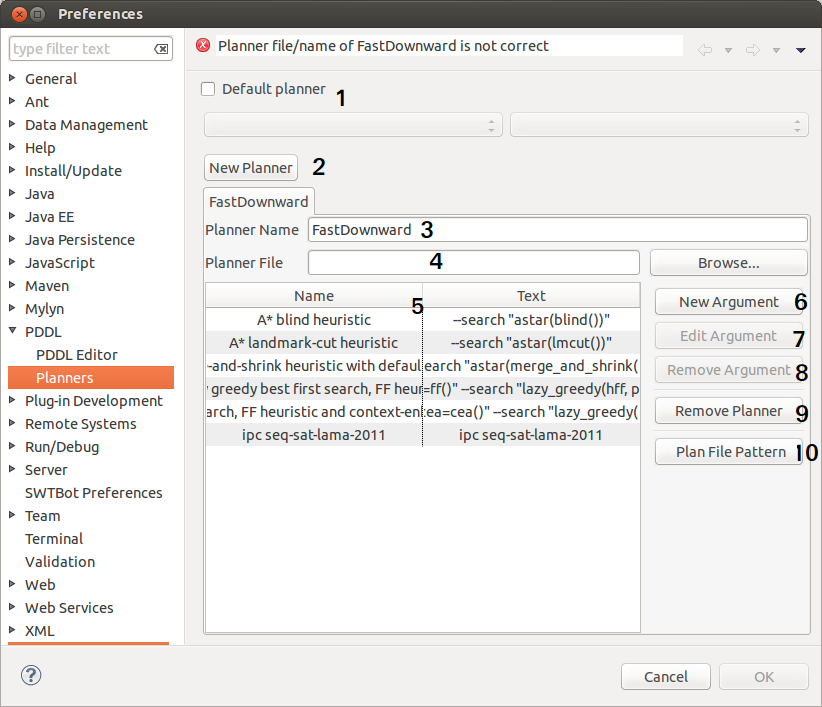
\includegraphics[width=\textwidth]{img/planner_preferences_window}
    \caption{Widok okna konfiguracji plannera.}
    \label{fig:preferences_window}
\end{figure}
Standardowo, dostępny jest wstępnie skonfigurowany planner \textit{FastDownward}. Okno preferencji udostępnia następujące opcje:
\begin{enumerate}
\item Wybór plannera domyślnego. Włączenie tej opcji, powoduje, że przy każdym uruchomieniu procesu planowania na plikach domeny i problemu, wykorzystany będzie wskazany w tym polu planner wraz z odpowiednim algorytmem planowania.
\item Nowa konfiguracja. Przycisk ten umożliwia stworzenie nowej konfiguracji, dla innego niż bieżący plannera. Może istnieć wiele takich konfiguracji, które w trakcie uruchamiania procesu planowania można dowolnie zmieniać.
\item Nazwa konfiguracji. Pozwala na rozróżnienie poszczególnych konfiguracji. Nazwa powinna być unikalna i może składać się z liter, cyfr, spacji oraz znaków ,,.'', ,,\_'', ,,-''.
\item Ścieżka do pliku plannera. Za pomocą przycisku \textit{Browse...} należy wskazać ścieżkę do pliku wykonywalnego lub skryptu powłoki systemu operacyjnego (\textit{Linux} lub \textit{Windows}), zgodnego z formatem przedstawionym w rozdziale~\ref{sec:wspolpraca}.
\item Argumenty plannera. W pierwszej kolumnie znajduje się czytelna dla użytkownika nazwa argumentu, w szczególności nazwa wykorzystywanego algorytmu planowania, która będzie używana jako prosty odpowiednik argumentu linii poleceń, znajdującego się w drugiej kolumnie. Parametry wiersza poleceń danego plannera wpisane muszą być w sposób identyczny, jak przy wpisywaniu ich podczas uruchamiania w konsoli.
\item Nowy argument. Przycisk ten umożliwia dodanie nowego argumentu linii poleceń plannera wraz z jego nazwą.
\item Edycja argumentu. Pozwala na edycję aktualnie zaznaczonego argumentu plannera.
\item Usunięcie argumentu. Pozwala na usunięcie aktualnie zaznaczonego argumentu plannera.
\item Usunięcie konfiguracji plannera. Przycisk ten usuwa bieżącą konfigurację. Nie ma możliwości cofnięcia tej operacji, dlatego przed jej wykonaniem wyświetlone zostaje pytanie, potwierdzające chęć usunięcia konfiguracji.
\item Wzorzec pliku planu. Okno to umożliwia zdefiniowanie wyrażenia regularnego, dotyczącego nazwy pliku wynikowego planu, powstałego w rezultacie działania bieżącego plannera. Prawidłowy wzorzec pozwala na wykrycie plików planów i bezpośrednie ich wyświetlenie przy pomocy przeglądarki planów (roz.~\ref{subsec:uruchamianie}).
\begin{figure}[h!]
    \centering
    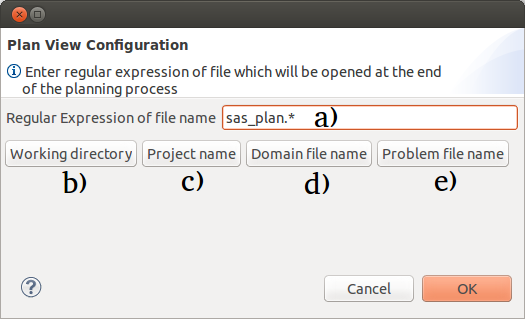
\includegraphics[width=0.8\textwidth]{img/plan_view_dialog}
    \caption{Widok okna konfiguracji przeglądarki planów.}
    \label{fig:plan_view_window}
\end{figure}
\begin{enumerate}
\item Wyrażenie regularne. Wzorzec opisujący nazwę pliku wynikowego planu. Planner \textit{FastDownward} standardowo generuje pliki planów o nazwie \texttt{sas\_plan.}, a w przypadku większej ilości planów kolejno \texttt{sas\_plan.1}, \texttt{sas\_plan.2}..., dlatego wyrażenie obejmujące te nazwy ma postać \texttt{sas\_plan.*}. Dla narzędzia \textit{SATPLAN} wzorzec ma postać \texttt{-problem\_file\_name-\textbackslash.pddl\textbackslash.soln} (opis wzorca \texttt{-problem\_file\_name-} znajduje się poniżej), ponieważ generuje pliki o nazwie \texttt{<nazwa\_pliku\_problemu>.pddl.soln}.
\item Wzorzec katalogu roboczego. Przycisk ten powoduje wstawienie w bieżącym miejscu kursora, ciągu \texttt{-working\_directory-}, który w czasie procesu planowania zamieniany jest na aktualną nazwę katalogu roboczego plannera (roz.~\ref{subsec:uruchamianie}). Opcja ta pozwala na wykrycie plików wynikowych, które jako swoją nazwę przyjmują nazwę bieżącego katalogu.
\item Wzorzec nazwy projektu. Przycisk ten powoduje wstawienie w bieżącym miejscu kursora, ciągu \texttt{-project\_name-}, który w czasie planowania zamieniany jest na nazwę projektu \textit{Eclipse}, w którym znajdują się przetwarzane pliki domeny oraz problemu.
\item Wzorzec nazwy pliku domeny. Przycisk ten powoduje wstawienie w bieżącym miejscu kursora, ciągu \texttt{-domain\_file\_name-}, który w czasie planowania zamieniany jest na nazwę pliku domeny, wykorzystywanej w tym przetwarzaniu, bez rozszerzenia \texttt{.pddl}.
\item Wzorzec nazwy pliku problemu. Przycisk ten powoduje wstawienie w bieżącym miejscu kursora, ciągu \texttt{-problem\_file\_name-}, który w czasie planowania zamieniany jest na nazwę pliku problemu, wykorzystywanego w tym przetwarzaniu, bez rozszerzenia \texttt{.pddl}.
\end{enumerate}
\end{enumerate}

Minimalna konfiguracja plannera, możliwa do zapisu składa się z prawidłowej nazwy oraz ścieżki do pliku programu. Zachowanie utworzonych lub zmodyfikowanych ustawień odbywa się po naciśnięciu przycisku ,,OK''.
Wszystkie konfiguracje zapisywane są w tzw. obszarze stanu (ang. \textit{state area}) przestrzeni roboczej (ang. \textit{workspace}) w folderze \path{planner_preferences}. 

Ścieżka do tego katalogu ma następującą postać:

\noindent
\centerline{\path{<l_p_rob>/.metadata/.plugins/pl.poznan.put.cs.gui4pddl/planner_preferences}}

\noindent
gdzie:

\noindent
\textbf{\path{<l_p_rob>}} -- lokalizacja przestrzeni roboczej.

Każda konfiguracja ustawień plannera zapisywana jest w osobnym pliku o nazwie analogicznej do wpisanej w oknie preferencji. Ze względu na łatwość modyfikacji, elastyczność w przechowywaniu listy argumentów oraz odporność na zmiany, jako format zapisu danych wybrano \textit{XML}. Do tego typu serializacji, wykorzystane zostało \textit{API} dołączone do platformy \textit{Eclipse} -- \textit{Memento}. W tej formie zapisywane są wszystkie informacje o konfiguracji, z wyjątkiem ustawień domyślnego plannera, które zachowywane są przy pomocy standardowego \textit{API} \textit{Eclipse} do zapisu preferencji -- \textit{Preferences}.

\lstset{language=XML}          % Set your language (you can change the language for each code-block optionally)
\begin{lstlisting}[frame=single,label={lst:preferencje_plannera},caption={Przykładowa konfiguracja plannera FastDownward w postaci XML}]  % Start your code-block
<?xml version="1.0" encoding="UTF-8"?>
<PlannerPreferences 
	PlanViewFilePattern="sas_plan.*" 
	PlannerFilePath="/home/user/fast-downward/src/plan" 
	PlannerName="FastDownward">
	<PlannerArguments>
		<PlannerArgumentsEntry 
			PlannerArgumentKey="A* blind heuristic" 
			PlannerArgumentValue="--search &quot;astar(blind())&quot;"/>
		<PlannerArgumentsEntry 
			PlannerArgumentKey="ipc seq-sat-lama-2011" 
			PlannerArgumentValue="ipc seq-sat-lama-2011"/>
	</PlannerArguments>
</PlannerPreferences>
\end{lstlisting}

\subsection{Uruchamianie zewnętrznego oprogramowania}
\label{subsec:uruchamianie}

Inicjalizacja oprogramowania wyznaczającego plan odbywa się poprzez wbudowany w \textit{Eclipse} mechanizm skrótów uruchamiania (ang \textit{Launch Shortcuts}). Rozszerzenie wtyczki o tego typu element pozwala na wywołanie zewnętrznych narzędzi przy pomocy menu \textit{Run} lub \textit{Debug}, a także przycisku znajdującego się na pasku narzędziowym lub menu kontekstowego edytowanego pliku.
\begin{figure}[h!]
    \centering
    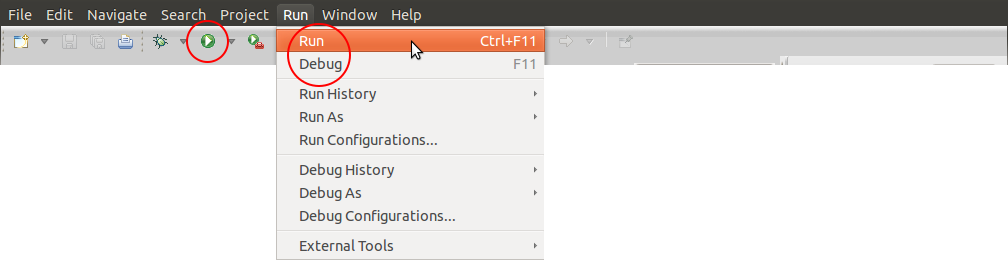
\includegraphics[width=0.9\textwidth]{img/running_options_menu_toolbar}
    \caption{Możliwość uruchomienia zewnętrznego oprogramowania z poziomu menu ,,Run'' oraz przycisku na pasku narzędziowym.}
    \label{fig:running_options_menu_toolbar}
\end{figure}

\begin{figure}[h!]
    \centering
    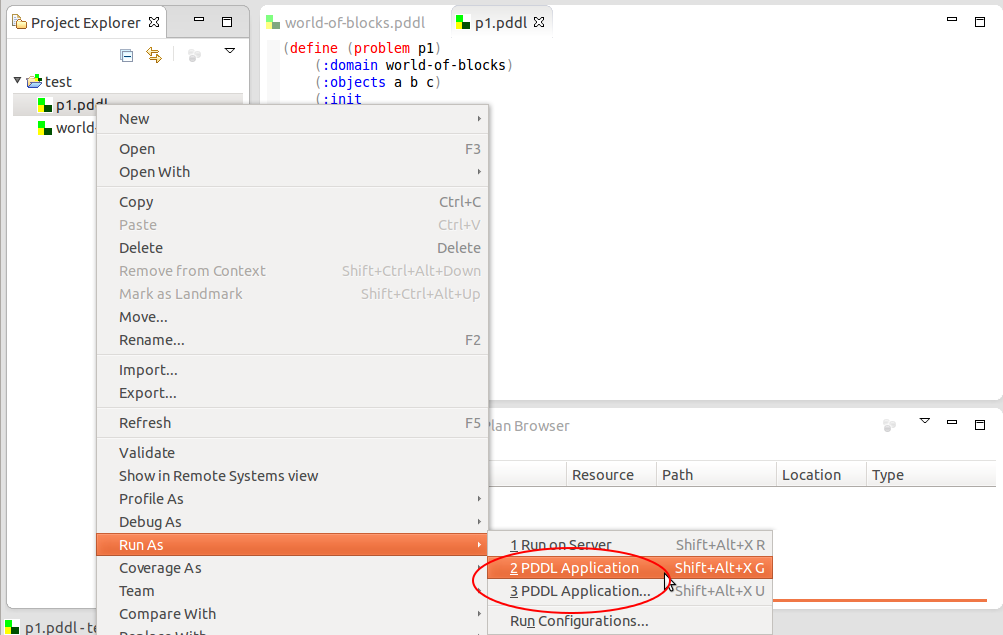
\includegraphics[width=0.9\textwidth]{img/running_options_context_menu}
    \caption{Możliwość uruchomienia zewnętrznego oprogramowania z poziomu menu kontekstowego edytowanego pliku.}
    \label{fig:running_options_context_menu}
\end{figure}

Podczas pierwszego uruchomienia zewnętrznego programu na aktualnie edytowanych plikach, tworzona jest nowa konfiguracja uruchamiania (ang. \textit{Run Configuration}). W przypadku, gdy opcja zastosowania domyślnego plannera (konfiguracja plannera, roz. \ref{subsec:konfiguracja}) nie jest ustawiona, należy w wyświetlonym oknie (rys. \ref{fig:run_configuration_window}) uzupełnić tę konfigurację o nazwę i argument plannera, który będzie wykorzystany w procesie planowania. 

\begin{figure}[h!]
    \centering
    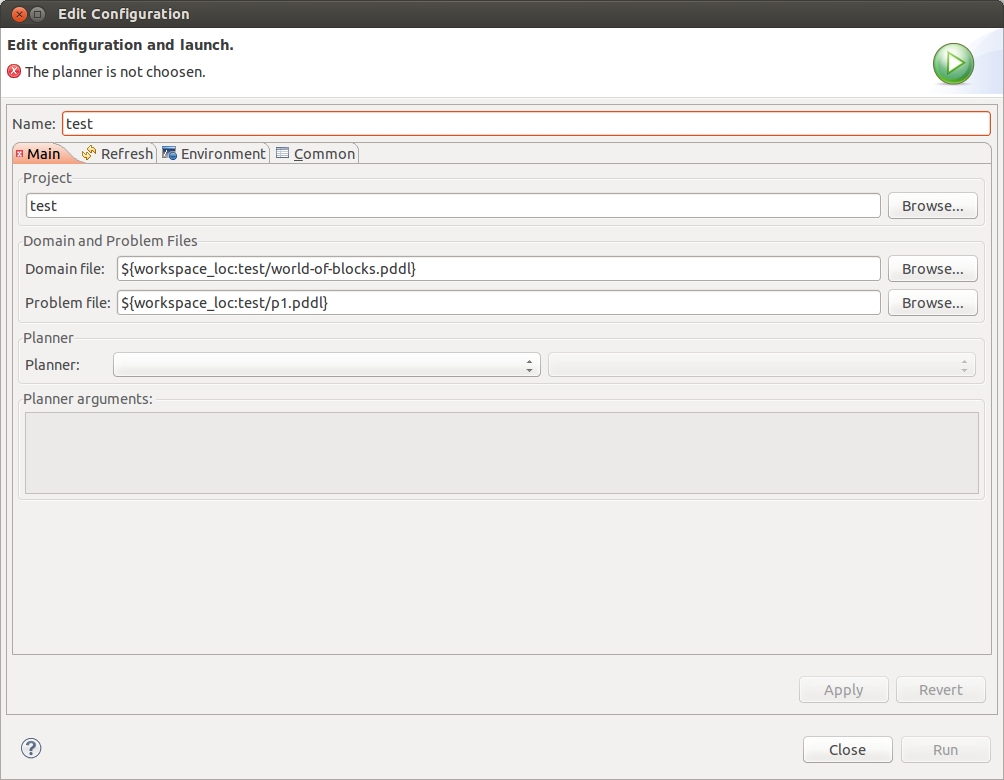
\includegraphics[width=0.9\textwidth]{img/run_configuration_window}
    \caption{Okno konfiguracji uruchamiania.}
    \label{fig:run_configuration_window}
\end{figure}

Jeżeli uruchomienie nastąpiło na pliku problemu (za pomocą globalnego menu \textit{Run} lub przycisku na pasku narzędziowym, gdy plik problemu był otwarty w edytorze, bądź poprzez wybranie z menu kontekstowego pliku problemu opcji \textit{Run as}, \textit{PDDL Project}) ścieżka do odpowiadającego pliku domeny w projekcie zostanie automatycznie wykryta za pomocą \textbf{INDEKSU KODU?} opisanego w rozdziale \textbf{ROZDZIAL}. Analogicznie w przypadku uruchomienia narzędzia na pliku domeny. W sytuacjach wyjątkowych (brak odpowiadającej domeny, więcej niż jeden pasujący problem) wyświetlane są listy wyboru:
\begin{itemize}
\item W przypadku gdy do danej domeny pasuje wiele plików problemów, wyświetla się okno wyboru ze wszystkimi pasującymi problemami.
\item W przypadku gdy do danej domeny nie pasuje żaden plik problemu, wyświetli się informująca o tym wiadomość.
\item W przypadku gdy do danego pliku problemu nie pasuje żaden plik domeny, ale w projekcie istnieją inne pliki domen, wyświetli się okno wyboru z wszystkimi plikami domen w projekcie.
\item W przypadku gdy do danego pliku problemu nie pasuje żaden plik domeny, ponieważ w projekcie nie istnieje żaden plik domeny, wyświetli się informująca o tym wiadomość.
\end{itemize}

Proces planowania rozpoczyna się po wybraniu przycisku \textit{Run} w oknie konfiguracji uruchamiania (lub z pominięciem tego okna w przypadku włączenia opcji domyślnego plannera w konfiguracji plannera). Działanie plannera objawia się widocznym paskiem postępu w prawym dolnym rogu aplikacji oraz na zakładce \textit{Progress} (rys.~\ref{fig:run_progress}). Również strumień wyjściowy działającego narzędzia kierowany jest w całości do widoku \textit{Console}.

\begin{figure}[h!]
    \centering
    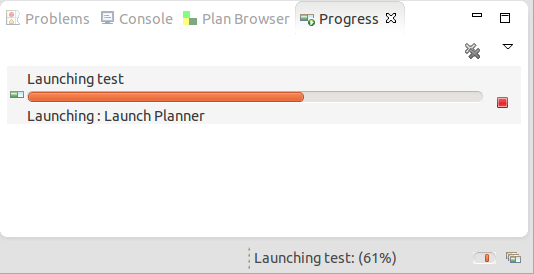
\includegraphics[width=0.8\textwidth]{img/run_progress}
    \caption{Pasek postępu procesu planowania.}
    \label{fig:run_progress}
\end{figure}

W razie błędów należy sprawdzić wyjście (w widoku \textit{Console}) oraz poprawność skryptu poprzez uruchomienie go w konsoli systemowej. Dobrą praktyką jest również zmiana ścieżki do przestrzeni roboczej \textit{Eclipse} w taki sposób, by nie zawierała spacji, gdyż niektóre narzędzia (np. \textit{SATPLAN}) niepoprawnie obsługują takie ścieżki.

Efektem przetwarzania jest powstanie planu, który w \textit{Eclipse} jest dostępny z poziomu przeglądarki planów (ang. \textit{Plan Browser}). Jest ona widoczna standardowo w pespektywie \textit{PDDL}, jako zakładka w dolnej części aplikacji. Każdy wiersz przeglądarki wskazuje na zakończony (powodzeniem lub niepowodzeniem) proces planowania. 

\begin{figure}[h!]
    \centering
    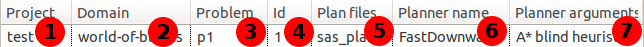
\includegraphics[width=0.9\textwidth]{img/plan_browser_row}
    \caption{Wiersz przeglądarki planów.}
    \label{fig:plan_browser_row}
\end{figure}

\noindent
Poszczególne kolumny oznaczają:
\begin{enumerate}
\item Nazwa projektu, który zawiera rozważany problem automatycznego planowania.
\item Nazwa domeny wykorzystywanej w rozważanym problemie automatycznego planowania. Standardowo jest to nazwa pliku domeny bez rozszerzenia \texttt{.pddl}.
\item Nazwa problemu wykorzystywanego w rozważanym problemie automatycznego planowania. Standardowo jest to nazwa pliku problemu bez rozszerzenie \texttt{.pddl}.
\item Numer ID przetwarzanego zadania o danej nazwie domeny i problemu, znajdującego się w danym projekcie. W celu możliwości zachowania poprzednich wyników planowania, każde przetwarzanie wykonywane jest w innym folderze roboczym, do którego ścieżka ma postać:

\noindent
\centerline{\path{<l_p_rob>/<project_name>/plans/<domain_name>/<problem_name>/<id>}}

\noindent
gdzie:

\begin{itemize}
\item \textbf{\path{<l_p_rob>}} -- lokalizacja przestrzeni roboczej.
\item \textbf{\path{<project_name>}} -- nazwa projektu.
\item \textbf{\path{<domain_name>}} -- nazwa domeny.
\item \textbf{\path{<problem_name>}} -- nazwa problemu.
\item \textbf{\path{<id>}} -- numer ID kolejnego przetwarzania.
\end{itemize}
Dzięki takiej strukturze katalogu roboczego użytkownik nie nadpisze omyłkowo poprzednio utworzonych wyników planowania. W przeglądarce planów powstaje zaś chronologiczna lista kolejnych uruchomień plannera, którą można swobodnie zarządzać, w tym usuwać.
\item Nazwy plików wynikowych, zawierających plan, które dopasowane są do wyrażenia regularnego ustalanego podczas konfiguracji plannera (roz.~\ref{subsec:konfiguracja}). W przypadku, gdy przetwarzanie nie zwróci pasujących plików lub zostanie przerwane przed zakończeniem, wyświetlany jest w tym miejscu komunikat o braku danych wynikowych (\textit{No plan files}).
\item Nazwa plannera, wykorzystywanego podczas znajdowania planu. Nazwa ta jest definiowana przy jego konfiguracji (roz.~\ref{subsec:konfiguracja}).
\item Nazwa argumentu plannera, wykorzystywanego podczas znajdowania planu, ustalana przy jego konfiguracji (roz.~\ref{subsec:konfiguracja}).
\end{enumerate}

Dane przeglądarki zapisywane są po wyłączeniu \textit{Eclipse} oraz wczytywane podczas uruchamiania platformy za pomocą \textit{API} \textit{Memento} w postaci \textit{XML}, analogicznej jak przy zapisie preferencji plannera (przykład~\ref{lst:preferencje_plannera});

Przeglądarka planów poza możliwością utrzymywania historii przetwarzania, daje również możliwość otwierania plików wynikowych oraz katalogu roboczego, a także wyszukiwania istniejących rekordów i ich usuwania:

\begin{figure}[h!]
    \centering
    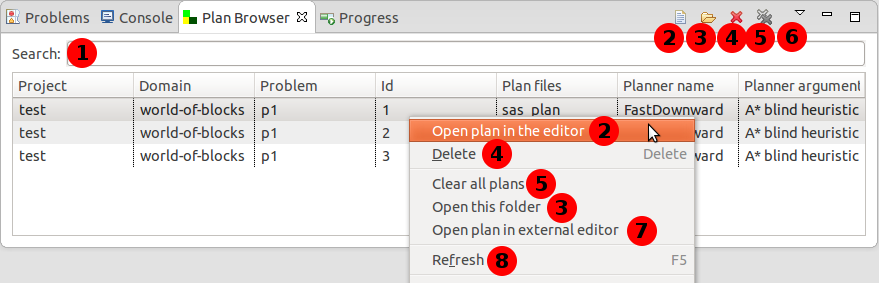
\includegraphics[width=\textwidth]{img/plan_browser_options}
    \caption{Dodatkowe opcje przeglądarki planów.}
    \label{fig:plan_browser_options}
\end{figure}

\begin{enumerate}
\item Wyszukiwarka rekordów, posiadająca możliwość prostego filtrowania wierszy, pasujących do zadanego wzorca.
\item Otwieranie pliku planu w wewnętrznym edytorze \textit{Eclipse}. W przypadku, gdy jest więcej niż jeden plik wynikowy, wyświetlona zostaje lista wyboru.
\item Otwieranie katalogu roboczego w systemowej przeglądarce plików, umożliwiające zarządzanie planami z poziomu plików, a także kontrolę błędów w przypadku nieprawidłowego przetwarzania.
\item Usunięcie zaznaczonego wiersza przeglądarki wraz z folderem roboczym, zawierającym wyniki przetwarzania, którego dotyczy ten rekord.
\item Usunięcie wszystkich rekordów przeglądarki wraz z odpowiadającymi im folderami roboczymi.
\item Wyłączenie/włączenie widoczności poszczególnych kolumn w tabeli przeglądarki.
\item Otwieranie pliku planu w standardowym edytorze tekstowym systemu operacyjnego. W przypadku, gdy jest więcej niż jeden plik wynikowy, wyświetlona zostaje lista wyboru.
\item Odświeżenie zawartości przeglądarki planów, pozwalające na usunięcie rekordów, dla których nie istnieją odpowiadające im pliki planów lub foldery robocze (ponieważ zostały wcześniej usunięte przez użytkownika z poziomu plików).
\end{enumerate}

Standardowym zachowaniem \textit{Eclipse} podczas inicjalizacji narzędzia zewnętrznego jest korzystanie z ostatnio utworzonej konfiguracji uruchamiania. Przy rozpoczęciu kolejnego procesu znajdowania planu na tych samych plikach, aplikacja nie wyświetla już okna edycji ustawień, lecz od razu przechodzi do fazy przetwarzania. Takie działanie daje użytkownikowi możliwość szybkiego sprawdzenia wyników planowania w trakcie edycji plików, lecz jednocześnie powoduje, że zmiana parametrów uruchamiania takich jak planner i jego argumenty jest utrudniona.

Z tego powodu utworzono dodatkową opcję edycji istniejących konfiguracji. Chcąc zmienić planner, bądź jego argumenty należy wybrać z menu kontekstowego edytowanego pliku element \textit{Run as} a następnie \textit{PDDL Project...} lub zastosować skrót klawiaturowy \texttt{Shift~+~Alt~+~X~+~U}. Gdy istnieje więcej niż jedna konfiguracja uruchamiania powiązana z danym plikiem, pojawi się okno wyboru istniejących profili (rys.~\ref{fig:run_configuration_choice}). Wybierając jeden z nich, użytkownik ma możliwość zmiany aktualnych parametrów.

\begin{figure}[h!]
    \centering
    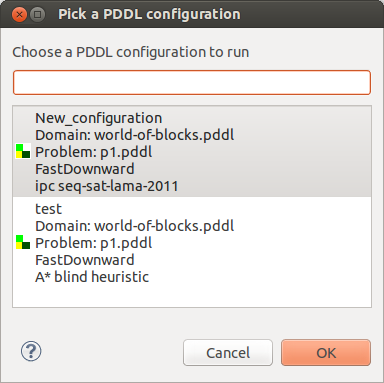
\includegraphics[width=0.5\textwidth]{img/run_configuration_choice}
    \caption{Okno wyboru istniejących konfiguracji uruchamiania.}
    \label{fig:run_configuration_choice}
\end{figure}

\subsection{Przerywanie procesu planowania}
\label{subsec:przerywanie}

Mnogość dostępnych narzędzi do wyznaczania planu, brak wśród nich jednoznacznego, powszechnie wykorzystywanego lidera oraz prawdopodobieństwo udoskonalania i powstawania nowych programów spowodowały, iż w projekcie GUI4PDDL powzięto założenie o wsparciu dla uruchamiania jak największego zakresu istniejących rozwiązań (z plannerem \textit{FastDownward} jako priorytetem). Wymaganie to zostało zrealizowane poprzez unifikację formatu pliku uruchomieniowego, obsługiwanego w \textit{Eclipse} (roz.~\ref{sec:wspolpraca}) oraz dostosowywanie do niego plannerów poprzez skrypty powłoki systemu operacyjnego.

Testy wykazały jednak, że środowisko programistyczne posiada kontrolę tylko nad procesami samych skryptów, natomiast wszystkie uruchamiane przez nie podprocesy (w tym proces programu plannera) pozostają bez nadzoru. W przypadku, gdy użytkownik zainicjalizuje kilka zadań znajdowania planu jednocześnie, które z uwagi na swój charakter i wykorzystywany algorytm znacznie obciążają procesor, może dojść do obniżenia responsywności systemu operacyjnego. Wówczas, mimo zatrzymania działania głównego skryptu za pomocą przycisku \textit{Terminate} w widoku \textit{Console}, procesy plannera nie zostaną zakończone, co może powodować dalszy spadek wydajności.

Rozwiązaniem tego problemu jest implementacja własnej fabryki procesów (ang. \textit{process factory}). Rozszerzenie to, wspierane przez platformę \textit{Eclipse}, pozwala na przejęcie kontroli nad tworzeniem nowego, natywnego procesu. W odpowiedzialnej za to metodzie \textit{newProcess} klasy \textit{PDDLProcessFactory} zwracany jest obiekt podklasy (\textit{RuntimeProcessWithChildProcessesTermination}) standardowego procesu, w której zmieniono część zajmującą się przerywaniem działania.

Nowy sposób zakończenia procesu opiera się na wykorzystaniu natywnych metod wspieranych systemów operacyjnych (\textit{Windows} oraz \textit{Linux}) poprzez bibliotekę \textit{JNA} (\textit{Java Native Access}). Biblioteka ta pozwala na wykonywanie operacji specyficznych dla danej platformy bez konieczności dodatkowej konfiguracji. Za jej pomocą pobierany jest numer \textit{PID} skryptu, który następnie podawany jest jako argument specyficznych dla systemu poleceń powłoki, odpowiedzialnych za przerywanie procesów. W przypadku systemu Windows jest to polecenie \textit{taskkill}, w przypadku rodziny \textit{Linux} -- \textit{kill}, z odpowiednio sparsowanym drzewem podprocesów otrzymanym z komendy \textit{pstree}.

Dzięki tak przygotowanemu wsparciu dla obsługi zakończenia skryptów, użytkownik jest w stanie kontrolować ich wykonywanie z poziomu \textit{Eclipse}, zarówno dla programów wsadowych (pliki \texttt{.bat} -- w systemie \textit{Windows}), jak i dla poleceń powłoki \textit{bash} (w systemach z rodziny \textit{Linux}).

\chapter{Testy}
\section{Testy jednostkowe kodu}

Aby wykryć i naprawić błędy, które znalazły się w kodzie projektu, przygotowano testy jednostkowe. Do wykonania testów użyto narzędzie \textit{JUnit }dostępne w środowisku programistycznym \textit{Eclipse}. Dodatkowo, aby sprawdzić pokrycie kodu testami, wykorzystano oprogramowanie \textit{Emma}.

Podczas prac nad projektem GUI4PDDL przetestowane zostały widoki oraz analizator składniowy. Testy pierwszego z dwóch wymienionych elementów polegały na prostym porównywaniu oczekiwanego stanu z stanem obecnym, za pomocą funkcji \textit{assertEquals}, która to należy do pakietu narzędzi \textit{JUnit}. Przykładowy, pojedynczy test przedstawiono w przykładzie \ref{test_jednostkowy}.\\\\
\begin{Code}
\begin{lstlisting}[language=JAVA,frame=single,label={test_jednostkowy}, caption={Przykładowy test jedostkowy}]
	@Test
	public void testGetRegexWithReplacementsAtBegin() {
		
		assertEquals(FileNameRegexProcessor.getRegexWithReplacements(
			"-project_name-projekt", "-project_name-", 
			"project-name"), "project-nameprojekt");
	}
\end{lstlisting}
\end{Code}


Testowanie analizatora składniowego polegało, przede wszystkim, na sprawdzeniu poprawności działania indeksowania poszczególnych elementów języka PDDL. Pierwszą czynnością jaką należało wykonać było wczytanie przykładowego pliku zawierajace go przykładową domenę. Następnie indeksowano plik za pomocą napisanej funkcji, dzięki czemu otrzymywano obiekt zawierający domenę wraz z jej zawartością. Dalej, tworzono pusty obiekt domeny, do którego kolejnymi instrukcjami oraz funkcjami dostarczonymi przez klasę, dołączano elementy znajdujące się w pliku. Porównanie tych dwóch obiektów zapewniało kompletną informację o działaniu indeksera.

Oprócz wyżej wymienionych testów, stworzono również badania pojedynczych funkcji znajdujących się w różnych miejscach kodu.

Testy jednostkowe wykryły kilka pomniejszych błędów, które należało usunąć. Spowodowane były one niepoprawnym indeksowaniem niektórych elementów języka PDDL. Przykładowo, testów nie przechodził kod, w którym zdefiniowano akcję zawierającą dyrektywę \textit{forall}.
\section{Testy jednostkowe gramatyk formalnych}
Oprócz standardowych testów jednostkowych, wymagane było przetestowanie gramatyki formalnej zawartej w projekcie GUI4PDDL. Jednym z sposobów przeprowadzenia testów jest wykorzystanie narzędzia \textit{GUnit}. Jest to specjalna platforma, wyspecjalizowana w tworzeniu testów gramatyk. Dzięki wbudowanym funkcjom \textit{GUnit} zmienia każdy z testów w instancje testu \textit{JUnit}, który następnie wykonywany jest standardowo przez odpowiedzialne narzędzie.

Aby testy gramatyki były kompletne, należało przetestować wszystkie zdefiniowane elementy języka PDDL. Opisano je w rozdziale \ref{sec:jezykpddl}. Są to między innymi akcje, wymagania, czy cele. W projekcie GUI4PDDL definicja gramatyki formalnej jest jednym z ważniejszych elementów, więc to dla niej przeznaczoną większą część testów.

Przykład \ref{gramatyka_formalna} przedstawia fagment gramatyki formalnej.


\begin{Code}
\begin{lstlisting}[language=LISP,frame=single,label={gramatyka_formalna}, caption={Fragment gramatyki formalnej}]
action_def 
	:	'(' ':action' NAME
			':parameters' '(' typed_list_of_variable ')'
			action_def_body_item* ')'   -> ^(':action' NAME ^(':parameters' 
				typed_list_of_variable)	action_def_body_item*) 
	;
\end{lstlisting}
\end{Code}

\begin{Code}
\begin{lstlisting}[language=LISP,frame=single,label={test_gramatyki}, caption={Przykładowe testy dla przykładu \ref{gramatyka_formalna}}]
<<
(:action load
        :parameters (?e - engine ?c - car ?t - town ?x - cargo)
        :precondition (and
            (cargo-at ?x ?t)
            (car-at ?c ?t)
            (not (exists (?y - cargo) (cargo-in ?y ?c)))
            )
        :effect (and
            (not (cargo-at ?x ?t))
            (cargo-in ?x ?c))
    )
>> OK


<<
(((()
>> FAIL
\end{lstlisting}
\end{Code}

Przykład 6.3 przedstawia fragment testu, dotyczącego elementu akcji. Każdy z testów otoczony jest znakami \texttt{<<} \texttt{>>}, po których następuje słowo \texttt{FAIL} bądź \texttt{OK}. To, które z tych dwóch słów znajduje się na końcu, określa czy testowany kod jest poprawny (\texttt{OK}) lub nie (\texttt{FAIL)}.




\section{Testy akceptacyjne}
W końcowym etapie tworzenia projektu GUI4PDDL podjęto testy akceptacyjne, mające na celu sprawdzenie spełnienia wymagań funkcjonalnych. Kolejne testy przedstawiono jako scenariusze i oczekiwane wyniki przeprowadzonych akcji.
Dodatkowo każde opisane zadanie zostało postawione przed potencjalnymi użytkownikami wtyczki GUI4PDDL, w celu sprawdzenia, czy projekt spełnia założenia dotyczące użytkowania praktycznego. Na końcu każdego scenariusza przedstawione zostały wnioski z obserwacji. 
\subsection{Utworzenie nowego projektu PDDL}
\textbf{Scenariusz testowy:}
  \begin{enumerate}
  
\item W środowisku \textit{Eclipse} należy kliknąć prawym przyciskiem myszy na polu \textit{Package Explorer} i wybrać \textit{New}, \textit{Other...} .
\item Wybrać z listy \textit{GUI4PDDL}, \textit{PDDL Project} i kliknąć \textit{Next}.
\item Wpisać nazwę projektu i kilknąć \textit{Finish}.
\end{enumerate}

\textbf{Oczekiwany wynik:} Na polu \textit{Package Explorer} powinien pojawić się nowy projekt o wybranej wcześniej nazwie.

\textbf{Obserwacja użytkowników:} Utworzenie nowego projektu PDDL nie powodowało problemów, nawet dla użytkowników nie znających środowiska \textit{Eclipse}.
\subsection{Dodanie nowego pliku do projektu PDDL}
\textbf{Scenariusz testowy:}
  \begin{enumerate}
  
\item Z pola \textit{Package Explorer} kliknąć prawym przyciskiem myszy na projekt PDDL. Wybrać \textit{New}, \textit{Other...} .
\item Wybrać z listy \textit{GUI4PDDL}, \textit{PDDL File} i kliknąć \textit{Next}.
\item W polu oznaczonym \textit{File name} wpisać nazwę i kliknąć \textit{Finish}.
\end{enumerate}

\textbf{Oczekiwany wynik:} W oknie głównym powinien pojawić się nowy plik. Po rozwinięciu zawartości projektu na polu \textit{Package Explorer}, również powinien być widoczny utworzony plik.

\textbf{Obserwacja użytkowników:} Dodawanie nowych plików nie stwarzało problemów osobom znającym środowisko \textit{Eclipse}. Pozostałe osoby potrzebowały chwilę czasu, aby zaznajomić się ze środowiskiem.  

\subsection{Dodawanie nowego planisty \textit{Fast Downward}}
\textbf{Scenariusz testowy:}
  \begin{enumerate}
  
\item W środowisku \textit{Eclipse}, wybrać listę rozwijaną \textit{Window} i wybrać \textit{Preferences}.
\item Z listy znajdującej się w oknie wybrać PDDL, a następnie \textit{Planners}.
\item W polu o etykiecie \textit{Planner File} podać lokalizację pliku planisty.
\item Zatwierdzić przyciskiem \textit{OK}.
\end{enumerate}

\textbf{Oczekiwany wynik:} Przy opcjach wyboru planisty powinna pojawić się możliwość wyboru \textit{Fast Downward}.

\textbf{Obserwacja użytkowników:} Osoby testujące nie potrafiły dodać nowego planisty bez wyraźnych instrukcji, nawet w sytuacji, gdy komunikat o błędzie wyraźnie wskazywał to miejsce. Wymagana jest dokładna dokumentacja opisująca poszczególne kroki dodawania nowego planisty. 
\subsection{Zmiana kolorów edytowanego kodu}
\textbf{Scenariusz testowy:}
  \begin{enumerate}
  
\item W środowisku \textit{Eclipse}, wybrać listę rozwijaną \textit{Window} i wybrać \textit{Preferences}.
\item Z listy znajdującej się w oknie wybrać PDDL, a następnie \textit{PDDL Editor}.
\item Przy odpowiednim elemencie kodu, kliknąć na pole z kolorem.
\item Wybrać odpowiedni kolor i zatwierdzić przyciskiem \textit{OK}.
\item Powtórzyć dla kolejnych elementów.
\item Zatwierdzić wszystkie zmiany przyciskiem \textit{Apply} bądź \textit{OK}.

\end{enumerate}

\textbf{Oczekiwany wynik:} W polu edycji kodu powinny uwidocznić się zmiany koloru elementów, których barwa została zmodyfikowana.

\textbf{Obserwacja użytkowników:} Sytuacja podobna do dodawania nowego planisty. Żadna z testowanych osób nie odnalazła w satysfakcjonującym czasie, opcji zmiany kolorów tworzonego kodu. Wynikało to z braku doświadczenia w tworzeniu oprogramowania w środowisku \textit{Eclipse}. Po odnalezieniu danych ustawień, użytkownicy wykonywali czynności płynnie i szybko. 
\subsection{Pierwsze uruchomienie planisty}
\textbf{Scenariusz testowy:}
  \begin{enumerate}
  
\item Należy wykonać czynności opisane w podrozdziałach 6.3.1, 6.3.2 oraz 6.3.3.
\item Wybrać domyślny przycisk służący w środowisku \textit{Eclipse} do uruchamiania tworzonego kodu.
\item W oknie, wybrać plik domeny, problemu oraz planistę wraz z algorytmem.
\item Zatwierdzić przyciskiem \textit{OK}. 
\end{enumerate}

\textbf{Oczekiwany wynik:} Wybrany planista powinien rozwiązać danych problem i wyświetlić dostępny wynik zakładce \textit{Plan Browser}. Otwarcie wyniku spowoduje wyświetlenie ułożonego planu na głównym polu. W przypadku gdy pliki są niepoprawne, informacje o błędach zostaną wyświetlone w zakładce \textit{Console}. 

\textbf{Obserwacja użytkowników:} Pierwsze uruchomienie planisty zajmowało więcej czasu niż jest to potrzebne doświadczonemu programiście. Powodem jest brak wyraźnego komunikatu, dotyczącego braku poszczególnych ustawień (np. brak pliku domeny czy problemu).




\chapter{Podsumowanie}
\label{sec:podsumowanie}
W prezentowanej pracy zaprojektowano oraz zaimplementowano graficzne narzędzie do opisu problemów planowania
w języku \emph{PDDL}.
Posiada ono funkcjonalność zintegrowanego środowiska programistycznego. Umożliwia tworzenie i zarządzanie
projektami oraz plikami \emph{PDDL}. W skład narzędzia wchodzą edytor strukturalny, moduł analizy kodu oraz moduł
integracji z zewnętrznym oprogramowaniem planisty. Wśród zaimplementowanych funkcji można wymienić: kolorowanie kodu źródłowego, znajdowanie błędów składniowych i semantycznych,
podpowiadanie składni, proste uruchamianie planisty, przeglądanie wyznaczonych planów.

Cel pracy, opisany w rozdziale 1.1, został spełniony. Zaimplementowano wszystkie funkcje, których specyfikacja
została zamieszczona w rozdziale 3.1. Automatyczne testy jednostkowe oraz ręczne testy integracyjne wykazały
poprawność i stabilność pracy oprogramowania. Wymagania pozafunkcjonalne zostały spełnione.

Narzędzie \emph{GUI4PDDL} zostało zaimplementowane jako wtyczka do środowiska Eclipse. Dzięki temu 
zespół miał możliwość zapoznania się z architekturą rozbudowanej aplikacji. Jest to cenne doświadczenie,
które może zostać wykorzystane w pracy zawodowej.

Planowane jest wykorzystanie opracowanego narzędzia na zajęciach dydaktycznych prowadzonych na Wydziale 
Informatyki Politechniki Poznańskiej w ramach przedmiotu Sztuczna Inteligencja. Opiekun niniejszej pracy mgr Jędrzej
Potoniec prowadzi zajęcia laboratoryjne z tego przedmiotu. Wprowadzenie zintegrowanego środowiska programistycznego
ułatwi studentom tworzenie i testowanie problemów planowania. Przyczyni się to do lepszego zrozumienia tematyki
automatycznego planowania.

Opracowane oprogramowanie posiada modułową strukturę. Dzięki temu w łatwy sposób może zostać dostosowane do 
nowych wymagań.

Wśród możliwości przyszłej rozbudowy narzędzia warto wymienić moduł symulacji planów, pełniący rolę narzędzia
do usuwania błędów. Moduł mógłby umożliwiać wykonywanie ciągu akcji w trybie pracy krokowej.
Możliwa byłaby wizualizacja zbioru spełnionych predykatów oraz wskazanie akcji ze spełninymi warunkami wstępnymi.
Podobne funkcje, w odniesieniu do systemów eksperckich, zawiera narzędzie \emph{CLIPS}\footnote{http://clipsrules.sourceforge.net}.

Inną możlwiością przyszłego rozwoju oprogramowania jest dodanie wsparcia dla języków wywodzących się z PDDL.
Można do nich zaliczyć \emph{Probabilistic PDDL} \cite{ppddl}, \emph{PDDL+} \cite{pddlplus} i \emph{Web-PDDL}
\cite{webpddl}. 



\appendix
\chapter{Zawartość płyty CD}
Do dokumentu załączona jest płyta CD o następującej zawartości:
\begin{enumerate}
\item Kod źródłowy oprogramowania
\item Skompilowana wersja instalacyjna
\item Instrukcja instalacji
\item Praca dyplomowa w postaci pliku pdf
\item Praca dyplomowa w postaci źródłowej
\end{enumerate}


\backmatter

\begin{thebibliography}{1}
\bibitem{adl} Michael Gelfond, Vladimir Lifschitz. \emph{Action Languages} Linköping Electronic Articles in
Computer and Information Science
Vol. 3(1998): nr 16. Dostępne w http://citeseerx.ist.psu.edu/viewdoc/download?doi= 10.1.1.146.4665\&{}rep=rep1\&{}type=pdf [Dostęp 15.01.2014]

\bibitem{fastdownward} Dostępne w: http://www.fast-downward.org/ [Dostęp: 18.01.2014]
\bibitem{fastforward} Dostępne w: http://fai.cs.uni-saarland.de/hoffmann/ff.html [Dostęp: 18.01.2014]
\bibitem{lpg} Dostępne w: http://zeus.ing.unibs.it/lpg/ [Dostęp: 18.01.2014]
\bibitem{satplanprog} Dostępne w: http://www.cs.rochester.edu/users/faculty/kautz/satplan/index.htm [Dostęp: 18.01.2014]
\bibitem{fdalgorytm} Malte Helmert. \emph{The Fast Downward Planning System}. Journal of Artifcial Intelligence Research 26 (2006) 191-246. Dostępne w: https://www.jair.org/media/1705/live-1705-2731-jair.pdf [Dostęp: 18.01.2014]
\bibitem{pddlplus} Maria Fox, Derek Long. \emph{PDDL+ : Modelling Continuous Time-dependent Effects}. Dostępne w: http://citeseerx.ist.psu.edu/viewdoc/download?doi=10.1.1.15.5965 \&{}rep=rep1\&{}type=pdf [Dostęp: 18.01.2014]
\bibitem{webpddl} Dejing Dou. \emph{The Formal Syntax and Semantics of Web-PDDL} Dostępne w: http://aimlab.uoregon.edu/web-pddl.pdf [Dostęp: 18.01.2014]
\bibitem{satplan} Henry Kautz. \emph{SATPLAN04: Planning as Satisfiability.} 1992. Dostępne w:
http://www.tzi.de/~edelkamp/ipc-4/Proc/satplan04.pdf [Dostęp: 18.01.2014]
\bibitem{gavs} Dostępne w: http://www6.in.tum.de/~chengch/gavs/ [Dostęp: 18.01.2014]
\bibitem{npdl} Jeremy Frank, Ari Jonsson. \emph{Constraint-based Attribute and Interval Planning.} 2002. Dostępne w:
http://ti.arc.nasa.gov/m/pub-archive/313h/0313\%20\%28Frank\%29.pdf [Dostęp: 18.01.2014] 
\bibitem{ppddl} Hakan L. S. Younes, Michael L. Littman. \emph{PPDDL1.0: An Extension to PDDL for Expressing
Planning Domains with Probabilistic Effects.} 2004. Dostęp w: http://reports-archive.adm.cs.cmu.edu/anon/2004/CMU-CS-04-167.pdf [Dostęp: 18.01.2014]
\bibitem{pddl3.1}Daniel L. Kovacs. \emph{Complete BNF description of PDDL 3.1 (completely corrected).} 2011. Dostępny w: http://www.plg.inf.uc3m.es/ipc2011-deterministic/attachments/OtherContributions/kovacs-pddl-3.1-2011.pdf [Dostęp: 18.01.2014]
\bibitem{opt} Drew McDermott. \emph{OPT Manual.} 2005. Dostępny w: http://www.cs.yale.edu/homes/dvm/papers/opt-manual.pdf [Dostęp: 18.01.2014]
\bibitem{strips} Richard E. Fikes, Nils J. Nilsson. \emph{Strips: A new approach to the application of theorem proving to problem solving.} International Joint Conferences on Artificial Intelligence, 1971.
\bibitem{planning} I.Vlahavas, I.Refanidis. \emph{Planning and Scheduling.} Dostępny w: http://www.eetn.gr/index.php/eetn-publications/ai-research-in-greece/planning-and-scheduling [Dostęp: 18.01.2014]
\bibitem{compilers}A. Aho, R. Sethi, J. Ullman. \emph{Kompilatory. Reguły, metody i narzędzia}.
WNT, 2001.
\bibitem{pddl}M. Ghallab et al. \emph{PDDL -- The Planning Domain Definition Language. Version 1.2}.
AIPS Conference, 1998.
\bibitem{antlr}T.~Parr. \emph{The Definitive ANTLR Reference. Building Domain-Specific Languages}. 
The Pragmatic Bookshelf, 2007.
\bibitem{eclipseplugins}E.~Clayberg, D.~Rubel. \emph{Eclipse Plug-Ins (3 ed.)}. Addison-Wesley Professional, 2008. 
\bibitem{eclipseinaction}Eclipse in Action: A Guide for the Java Developer by \emph{David Gallardo}, Chapter 8,9
\bibitem{eclipsearticle} The Architecture of Open Source Application by Kim Moir Dostępne w http://www.aosabook.org/en/eclipse.html [Dostęp: 19.01.2014]
\end{thebibliography}


\end{document}
